\section{Experiments \label{sec-exp}}
%In this section, we will verify the superiority of HERec by performing experiments on three real datasets and comparing it to the state-of-the-arts.
%In this section, we construct the experimental evaluation and present the  result analysis.
In this section, we will demonstrate the effectiveness of HERec by performing experiments on three real datasets compared to the state-of-the-art recommendation methods.

\begin{table*}[t]%[htbp]
\centering
%\scriptsize
\caption{\label{tab_Data} Statistics of the three datasets.}
{
\begin{tabular}{|c||c|c|c|c|c|c|c|}
\hline
{Dataset} & {Relations} & {Number} & {Number} & {Number} & {Ave. degrees} & {Ave. degrees} & \multirow{2}{*}{Meta-paths}\\
{(Density)} & {(A-B)} & {of A} & {of B} & {of (A-B)}  & {of A} & {of B} &  \multirow{2}{*}{}\\
\hline
\hline
\multirow{6}{*}{Douban Movie} & {User-Movie} & {13,367} & {12,677} & {1,068,278} & {79.9} & {84.3} & {} \\
\cline{2-7}
\multirow{6}{*}{(0.63\%)} &  {User-User} & {2,440} & {2,294} & {4,085} & {1.7} & {1.8} & {UMU, MUM} \\
\cline{2-7}
\multirow{6}{*}{} &{User-Group} & {13,337} & {2,753} & {570,047} & {42.7} & {207.1} & {UMDMU, MDM}\\
\cline{2-7}
\multirow{6}{*}{} & {Movie-Director} & {10,179} & {2,449} & {11,276} & {1.1} & {4.6} & {UMAMU, MAM} \\
\cline{2-7}
\multirow{6}{*}{} & {Movie-Actor} & {11,718} & {6,311} & {33,587} & {2.9} & {5.3} & {UMTMU, MTM}\\
\cline{2-7}
\multirow{6}{*}{} & {Movie-Type} & {12,678} & {38} & {27,668} & {2.2} & {728.1} & {}\\
\hline
\hline
\multirow{5}{*}{Douban Book} & {User-Book} & {13,024} & {22,347} & {792,026} & {60.8} & {35.4} & \multirow{2}{*}{UBU, BUB} \\
\cline{2-7}
\multirow{5}{*}{(0.27\%)} & {User-User} & {12,748} & {12,748} & {169,150} & {13.3} & {13.3} & \multirow{2}{*}{UBPBU, BPB} \\
\cline{2-7}
\multirow{5}{*}{} & {Book-Author} & {21,907} & {10,805} & {21,905} & {1.0} & {2.0} & \multirow{2}{*}{UBYBU, BYB} \\
\cline{2-7}
\multirow{5}{*}{} & {Book-Publisher} & {21,773} & {1,815} & {21,773} & {1.0} & {11.9} & \multirow{2}{*}{UBABU} \\
\cline{2-7}
\multirow{5}{*}{} & {Book-Year} & {21,192} & {64} & {21,192} & {1.0} & {331.1} & \multirow{2}{*}{} \\
\hline
\hline
\multirow{5}{*}{Yelp} & {User-Business} & {16,239} & {14,284} & {198,397} & {12.2} & {13.9} &{} \\
\cline{2-7}
\multirow{5}{*}{(0.08\%)} & {User-User} & {10,580} & {10,580} & {158,590} & {15.0} & {15.0} &{UBU, BUB} \\
\cline{2-7}
\multirow{5}{*}{} & {User-Compliment} & {14,411} & {11} & {76,875} & {5.3} & {6988.6} & {UBCiBU, BCiB} \\
\cline{2-7}
\multirow{5}{*}{} & {Business-City} & {14,267} & {47} & {14,267} & {1.0} & {303.6} & {UBCaBU, BCaB} \\
\cline{2-7}
\multirow{5}{*}{} & {Business-Category} & {14,180} & {511} & {40,009} & {2.8} & {78.3} & {} \\
\hline

\end{tabular}}
\end{table*}

%\begin{table}[t]%[htbp]
%\center
%%\scriptsize
%\caption{\label{tab_metapath} The selected meta-paths for  three datasets in our work.}
%{\begin{tabular}{|c||c|}
%\hline
%{Dataset} & {Meta-paths}\\
%\hline\hline
%\multirow{2}{*}{Douban Movie} & {UMU, UMDMU, UMAMU, UMTMU}\\
%\multirow{2}{*}{} & {MUM, MAM, MDM, MTM} \\
%\hline
%\multirow{2}{*}{Douban Book} & {UBU, UBABU, UBPBU, UBYBU} \\
%\multirow{2}{*}{} & {BUB, BPB, BYB} \\
%\hline
%\multirow{2}{*}{Yelp} & {UBU, UBCiBU, UBCaBU} \\
%\multirow{2}{*}{} & {BUB, BCiB, BCaB} \\
%\hline
%\end{tabular}}
%\end{table}


\begin{table*}[t]
\centering
%\scriptsize
\caption{\label{tab_Effectiveness} Results of effectiveness experiments on three datasets. A smaller MAE or RMSE value indicates a better performance. For ease of reading the results, we also report the improvement w.r.t. the PMF model for each other method. A larger improvement ratio indicates a better performance. }
{
\begin{tabular}{|c|c|c||c|c|c|c|c|c||c|c||c|}
\hline
{Dataset} & {Training} & {Metrics}  & {PMF} &{SoMF} & {FM$_{HIN}$} & {HeteMF}& {SemRec}  & {DSR} & {HERec$_{dw}$} & {HERec$_{mp}$}&{HERec}\\
\hline
\hline
\multirow{16}{*}{Douban}& \multirow{4}{*}{80\%} & {MAE} & {0.5741} & {0.5817} & {0.5696} & {0.5750} & {0.5695} &  {0.5681}  & {0.5703} & {\textbf{0.5515}} &{0.5519} \\
\multirow{16}{*}{} &\multirow{4}{*}{}& {Improve} & {} & {-1.32\%} & {+0.78\%} & {-0.16\%} & {+0.80\%}  & {+1.04\%} & {+0.66\%} &{+3.93\%} & {+3.86\%} \\
\cline{3-12}
\multirow{16}{*}{Movie} &\multirow{4}{*}{}& {RMSE} & {0.7641} & {0.7680} &   {0.7248} & {0.7556}& {0.7399} & {0.7225} & {0.7446} & {0.7121} & {\textbf{0.7053}} \\
\multirow{16}{*}{} &\multirow{4}{*}{}& {Improve} & {} & {-0.07\%} & {+5.55\%} & {+1.53\%} & {+3.58\%}  & {+5.85\%} & {+2.97\%} &{+7.20\%} & {+8.09\%} \\
\cline{2-12}
\multirow{16}{*}{} &\multirow{4}{*}{}\multirow{4}{*}{60\%} & {MAE} & {0.5867} & {0.5991} & {0.5769} & {0.5894} & {0.5738} &  {0.5831} & {0.5838} & {0.5611} &{\textbf{0.5587}} \\
\multirow{16}{*}{} &\multirow{4}{*}{}& {Improve} & {} & {-2.11\%} & {+1.67\%} & {-0.46\%} & {+2.19\%}  & {+0.61\%} & {+0.49\%} &{+4.36\%} & {+4.77\%} \\
\cline{3-12}
\multirow{16}{*}{} &\multirow{4}{*}{}& {RMSE} & {0.7891} & {0.7950} & {0.7842} & {0.7785} & {0.7551} &  {0.7408} & {0.7670} & {0.7264} &{\textbf{0.7148}} \\
\multirow{16}{*}{} &\multirow{4}{*}{}& {Improve} & {} & {-0.75\%} & {+0.62\%} & {+1.34\%} & {+4.30\%}  & {+6.12\%} & {+2.80\%} &{+7.94\%} & {+9.41\%} \\
\cline{2-12}
\multirow{16}{*}{} &\multirow{4}{*}{}\multirow{4}{*}{40\%} & {MAE} & {0.6078} & {0.6328} &  {0.5871} & {0.6165} & {0.5945} &  {0.6170} & {0.6073} & {0.5747} &{\textbf{0.5699}}\\
\multirow{16}{*}{} &\multirow{4}{*}{}& {Improve} & {} & {-4.11\%} & {+3.40\%} & {-1.43\%} & {+2.18\%}  & {-1.51\%} & {+0.08\%} &{+5.44\%} & {+6.23\%} \\
\cline{3-12}
\multirow{16}{*}{} &\multirow{4}{*}{}& {RMSE} & {0.8321} & {0.8479} & {0.7563} & {0.8221} & {0.7836} &  {0.7850} & {0.8057} & {0.7429} &{\textbf{0.7315}} \\
\multirow{16}{*}{} &\multirow{4}{*}{}& {Improve} & {} & {-1.89\%} & {+9.10\%} & {+1.20\%} & {+5.82\%}  & {+5.66\%} & {+3.17\%} &{+10.71\%} & {+12.09\%} \\
\cline{2-12}
\multirow{16}{*}{} &\multirow{4}{*}{}\multirow{4}{*}{20\%} & {MAE}& {0.7247}& {0.6979} & {0.6080} & {0.6896} & {0.6392} &  {0.6584} & {0.6699} & {0.6063} &{\textbf{0.5900}} \\
\multirow{16}{*}{} &\multirow{4}{*}{}& {Improve} & {} & {+3.69\%} & {+16.10\%} & {+4.84\%} & {+11.79\%}  & {+9.14\%} & {+7.56\%} &{+16.33\%} & {+18.59\%} \\
\cline{3-12}
\multirow{16}{*}{} &\multirow{4}{*}{}& {RMSE} & {0.9440} & {0.9852} & {0.7878} & {0.9357} & {0.8599} &  {0.8345} & {0.9076} & {0.7877}  &{\textbf{0.7660}}\\
\multirow{16}{*}{} &\multirow{4}{*}{}& {Improve} & {} & {-4.36\%} & {+16.55\%} & {+0.88\%} & {+8.91\%}  & {+11.60\%} & {+3.86\%} &{+16.56\%}& {+18.86\%} \\


\hline
\hline
\multirow{16}{*}{Douban}& \multirow{4}{*}{80\%} & {MAE} & {0.5774} & {0.5756}  & {0.5716} & {0.5740}   & {0.5675}   &  {0.5740}    & {0.5875}   & {0.5591} &{\textbf{0.5502}} \\
\multirow{16}{*}{} &\multirow{4}{*}{}& {Improve} & {} & {+0.31\%} & {+1.00\%} & {+0.59\%} & {+1.71\%}  & {+0.59\%} & {-1.75\%} &{+3.17\%} & {+4.71\%} \\
\cline{3-12}
\multirow{16}{*}{Book} &\multirow{4}{*}{}& {RMSE}             & {0.7414} & {0.7302}   & {0.7199} & {0.7360}   & {0.7283}   &  {0.7206}    & {0.7450}  & {0.7081} &{\textbf{0.6811}}\\
\multirow{16}{*}{} &\multirow{4}{*}{}& {Improve} & {} & {+1.55\%} & {+2.94\%} & {+0.77\%} & {+1.81\%}  & {+2.84\%} & {-0.44\%} &{+4.53\%} & {+8.17\%} \\
\cline{2-12}
\multirow{16}{*}{} &\multirow{4}{*}{}\multirow{4}{*}{60\%} & {MAE} & {0.6065} & {0.5903}   &{0.5812} & {0.5823}   & {0.5833}   &  {0.6020}   & {0.6203}  & {0.5666} &{\textbf{0.5600}}\\
\multirow{16}{*}{} &\multirow{4}{*}{}& {Improve} & {} & {+2.67\%} & {+4.17\%} & {+3.99\%} & {+3.83\%}  & {+0.74\%} & {-2.28\%} &{+6.58\%} & {+7.67\%} \\
\cline{3-12}
\multirow{16}{*}{} &\multirow{4}{*}{}& {RMSE}    & {0.7908} & {0.7518}   &{0.7319} & {0.7466}   & {0.7505}   &  {0.7552}   & {0.7905}  & {0.7318} &{\textbf{0.7123}}\\
\multirow{16}{*}{} &\multirow{4}{*}{}& {Improve} & {} & {+4.93\%} & {+7.45\%} & {+5.59\%} & {+5.10\%}  & {+4.50\%} & {+0.04\%} &{+7.46\%} & {+9.93\%} \\
\cline{2-12}
\multirow{16}{*}{} &\multirow{4}{*}{}\multirow{4}{*}{40\%} & {MAE} & {0.6800} & {0.6161}   &{0.6028} & {0.5982}   & {0.6025}   &  {0.6271}   & {0.6976}  & {0.5954} &{\textbf{0.5774}}\\
\multirow{16}{*}{} &\multirow{4}{*}{}& {Improve} & {} & {+9.40\%} & {+11.35\%} & {+12.03\%} & {+11.40\%}  & {+7.78\%} & {-2.59\%} &{+12.44\%}& {+15.09\%} \\
\cline{3-12}
\multirow{16}{*}{} &\multirow{4}{*}{}& {RMSE}    & {0.9203} & {0.7936}   &{0.7617} & {0.7779}   & {0.7751}   &  {0.7730}   & {0.9022}  & {0.7703} &{\textbf{0.7400}}\\
\multirow{16}{*}{} &\multirow{4}{*}{}& {Improve} & {} & {+13.77\%} & {+17.23\%} & {+15.47\%} & {+15.78\%}  & {+16.01\%} & {+1.97\%} &{+16.30\%} & {+19.59\%} \\
\cline{2-12}
\multirow{16}{*}{} &\multirow{4}{*}{}\multirow{4}{*}{20\%} & {MAE}& {1.0344} & {0.6327}   &{0.6396} & {0.6311}   & {0.6481}   &  {0.6300}   & {1.0166}   & {0.6785}  &{\textbf{0.6450}}\\
\multirow{16}{*}{} &\multirow{4}{*}{}& {Improve} & {} & {+38.83\%} & {+38.17\%} & {+38.99\%} & {+37.35\%}  & {+39.10\%} & {+1.72\%} &{+34.41\%} & {+37.65\%} \\
\cline{3-12}
\multirow{16}{*}{} &\multirow{4}{*}{}& {RMSE}    & {1.4414} & {0.8236}   &{0.8188} & {0.8304}   & {0.8350}   &  {0.8200}   & {1.3205}   & {0.8869} &{\textbf{0.8581}} \\
\multirow{16}{*}{} &\multirow{4}{*}{}& {Improve} & {} & {+42.86\%} & {+43.19\%} & {+42.39\%} & {+42.07\%}  & {+43.11\%} & {+8.39\%} &{+38.47\%} & {+40.47\%} \\
%\cline{2-12}
%{} &\multicolumn{2}{c||}{Average Rank} & {8.88} & {5.88} & {5.50} & {5.53} & {4.88} & {8.75} & {2.25} & {2.37} & {\textbf{1.63}}\\
\hline
\hline
\multirow{16}{*}{Yelp}& \multirow{4}{*}{90\%} & {MAE} & {1.0412} & {1.0095}   &{0.9013} & {0.9487}   & {0.9043}   &  {0.9054}    & {1.0388}   & {0.8822} &{\textbf{0.8395}} \\
\multirow{16}{*}{} &\multirow{4}{*}{}& {Improve} & {} & {+3.04\%} & {+13.44\%} & {+8.88\%} & {+13.15\%}  & {+13.04\%} & {+0.23\%} &{+15.27\%} & {+19.37\%} \\
\cline{3-12}
\multirow{16}{*}{} &\multirow{4}{*}{}& {RMSE}             & {1.4268} & {1.3392}   &{1.1417} & {1.2549}   & {1.1637}   &  {1.1186}    & {1.3581}  & {1.1309}  &{\textbf{1.0907}}\\
\multirow{16}{*}{} &\multirow{4}{*}{}& {Improve} & {} & {+6.14\%} & {+19.98\%} & {+12.05\%} & {+18.44\%}  & {+21.60\%} & {+4.81\%} &{+20.74\%} & {+23.56\%} \\
\cline{2-12}
\multirow{16}{*}{} &\multirow{4}{*}{}\multirow{4}{*}{80\%} & {MAE} & {1.0791} & {1.0373}   &{0.9038} & {0.9654}   & {0.9176}   &  {0.9098}   & {1.0750}   & {0.8953}  &{\textbf{0.8475}} \\
\multirow{16}{*}{} &\multirow{4}{*}{}& {Improve} & {} & {+3.87\%} & {+16.25\%} & {+10.54\%} & {+14.97\%}  & {+15.69\%} & {+0.38\%} &{+17.03\%} & {+21.46\%} \\
\cline{3-12}
\multirow{16}{*}{} &\multirow{4}{*}{}& {RMSE}    & {1.4816} & {1.3782}   &{1.1497} & {1.2799}   & {1.1771}   &  {1.1208}   & {1.4075}   & {1.1516} &{\textbf{1.1117}}\\
\multirow{16}{*}{} &\multirow{4}{*}{}& {Improve} & {} & {+6.98\%} & {+22.40\%} & {+13.61\%} & {+20.55\%}  & {+24.35\%} & {+5.00\%} &{+22.27\%} & {+24.97\%} \\
\cline{2-12}
\multirow{16}{*}{} &\multirow{4}{*}{}\multirow{4}{*}{70\%} & {MAE} & {1.1170} & {1.0694}   &{0.9108} & {0.9975}   & {0.9407}   &  {0.9429}   & {1.1196}  & {0.9043} &{\textbf{0.8580}}\\
\multirow{16}{*}{} &\multirow{4}{*}{}& {Improve} & {} & {+4.26\%} & {+18.46\%} & {+10.70\%} & {+15.78\%}  & {+15.59\%} & {-0.23\%} &{+19.04\%} & {+23.19\%} \\
\cline{3-12}
\multirow{16}{*}{} &\multirow{4}{*}{}& {RMSE}    & {1.5387} & {1.4201}   &{1.1651} & {1.3229}   & {1.2108}   &  {1.1582}   & {1.4632}  & {1.1639}  &{\textbf{1.1256}}\\
\multirow{16}{*}{} &\multirow{4}{*}{}& {Improve} & {} & {+7.71\%} & {+24.28\%} & {+14.02\%} & {+21.31\%}  & {+24.73\%} & {+4.91\%} &{+24.36\%} & {+26.85\%} \\
\cline{2-12}
\multirow{16}{*}{} &\multirow{4}{*}{}\multirow{4}{*}{60\%} & {MAE}& {1.1778} & {1.1135}   &{0.9435} & {1.0368}   & {0.9637}   &  {1.0043}   & {1.1691}  & {0.9257}  &{\textbf{0.8759}}\\
\multirow{16}{*}{} &\multirow{4}{*}{}& {Improve} & {} & {+5.46\%} & {+19.89\%} & {+11.97\%} & {+18.18\%}  & {+14.73\%} & {+0.74\%} &{+21.40\%} & {+25.63\%} \\
\cline{3-12}
\multirow{16}{*}{} &\multirow{4}{*}{}& {RMSE}    & {1.6167} & {1.4748}   &{1.2039} & {1.3713}   & {1.2380}   &  {1.2257}   & {1.5182}   & {1.1887}  &{\textbf{1.1488}}\\
\multirow{16}{*}{} &\multirow{4}{*}{}& {Improve} & {} & {+8.78\%} & {+25.53\%} & {+15.18\%} & {+23.42\%}  & {+24.19\%} & {+6.09\%} &{+26.47\%} & {+28.94\%} \\
%\cline{2-12}
%{} &\multicolumn{2}{c||}{Average Rank} & {9.00} & {7.88} & {6.00} & {4.63} & {4.38} & {7.13} & {3.00} & {1.75} & {\textbf{1.25}}\\
\hline
%\hline
%\multicolumn{3}{|c||}{Average Rank} & {10.33} & {8.79} &{5.25} & {7.83} & {6.54} &  {6.13} & {9.5} & {4.17} & {3.2} & {2.4} & {\textbf{1.79}}\\
%\hline
\end{tabular}}
\end{table*}

\subsection{Evaluation Datasets}
We adopt three widely used datasets from different domains, consisting of Douban Movie dataset \footnote{http://movie.douban.com} from movie domain, Douban Book dataset \footnote{http://book.douban.com} from book domain, and Yelp dataset \footnote{http://www.yelp.com/dataset-challenge} from business domain. Douban Movie dataset includes 13,367 users and 12,677 movies with 1,068,278 movie ratings ranging from 1 to 5. Moreover, the dataset also includes social relations and attribute information of users and movies. As for the Douban Book dataset, it includes 13,024 users and 22,347 books with 792,026 ratings ranging from 1 to 5. Yelp dataset records user ratings on local businesses and contains social relations and attribute information of businesses, which includes 16,239 users and 14,282 local businesses with 198,397 ratings raging from 1 to 5. The detailed descriptions of the three datasets are shown in Table~\ref{tab_Data}, and the network schemas of the three datasets are plotted in Fig.~\ref{fig_schema}. Besides the domain variation, these three datasets also have different rating sparsity degrees: the Yelp dataset is very sparse, while the Douban Movie dataset is much denser.



\subsection{Metrics}
We use the widely used mean absolute error (MAE) and root mean square error (RMSE) to measure the quality of recommendation of different models. The metrics MAE and RMSE are defined as follows:

\begin{equation}
MAE = \frac{1}{|\mathcal{D}_{test}|}\sum_{(i, j) \in \mathcal{D}_{test}}{|r_{i,j} - \widehat{r_{i,j}}|},
\end{equation}
\begin{equation}
RMSE = \sqrt{\frac{1}{|\mathcal{D}_{test}|}\sum_{(i, j) \in \mathcal{D}_{test}}{(r_{i,j} - \widehat{r_{i,j}})^2}},
\end{equation}
where $r_{i,j}$ is the actual rating that user $i$ assigns to item $j$, $\widehat{r_{i,j}}$ is the predicted rating from a model, and $\mathcal{D}_{test}$ denotes the test set of rating records. From the definition, we can see that a smaller MAE or RMSE value indicates a better performance.

%\subsection{Evaluation Datasets and Metrics}
%
%We adopt three widely used datasets from different domains, including Douban Movie dataset \footnote{http://movie.douban.com}, Douban Book dataset \footnote{http://book.douban.com}, and Yelp dataset \footnote{http://www.yelp.com/dataset-challenge}. The detailed statistics of three datasets are
%summarized in Table~\ref{tab_Data}.
%We use two commonly adopted metrics to measure the performance of rating prediction, namely mean absolute error (MAE) and root mean square error (RMSE) \cite{willmott2005advantages}.


\subsection{Methods to Compare}
%In order to verify the effectiveness of HERec, we compare HERec with quite a few baselines, some of which represent state-of-the-art for HIN-based recommendation. Since there are three embedding fusion functions in HERec, we include three versions of HERec: HERec$_{sl}$, HERec$_{pl}$, and HERec$_{pnL}$. Moreover, we also design two methods, called HERec$_{dw}$ and HERec$_{mp}$, which replace our HIN embedding with two well known network embeddings under the framework of HERec. As the baselines, six representative rating predication methods are employed, including two classical matrix factorization methods (i.e., PMF and SoMF) and  four HIN based recommendation methods (FM$_{HIN}$, HeteMF, SemRec and DSR).
We consider the following methods to compare:

\textbullet\ \textbf{PMF}~\cite{mnih2008probabilistic}: It is the classic probabilistic matrix factorization model by explicitly factorizing the rating matrix into two low-dimensional matrices.

\textbullet\ \textbf{SoMF}~\cite{ma2011recommender}: It incorporates social network information into the recommendation model.
The social relations are characterized by a social regularization term, and integrated into the basic matrix factorization model.

\textbullet\ \textbf{FM$_{HIN}$}: It is the context-aware factorization machine~\cite{rendle2012factorization}, which is able to utilize various kinds of auxiliary information. In our experiments, we extract heterogeneous information as context features and incorporate them into the factorization machine for rating prediction. We implement the model with the code from the authors~\footnote{http://www.libfm.org/}.


\textbullet\ \textbf{HeteMF}~\cite{yu2013collaborative}: It is a MF based recommendation method, which utilizes entity similarities calculated over HINs using meta-path based algorithms.

\textbullet\ \textbf{SemRec}~\cite{shi2015semantic}: It is a collaborative filtering method on weighted heterogeneous information network, which is constructed by connecting users and items with the same ratings. It flexibly integrates heterogeneous information for recommendation by weighted meta-paths and a weight ensemble method. We implement the model with the code from the authors~\footnote{https://github.com/zzqsmall/SemRec}.


\textbullet\ \textbf{DSR}~\cite{zheng2017recommendation}: It is a MF based recommendation method with dual similarity regularization, which imposes the constraint on users and items with high and low similarities simultaneously.

\textbullet \textbf{HERec$_{dw}$}: It is a variant of HERec, which adopts the homogeneous network embedding method deepwalk~\cite{perozzi2014deepwalk} and ignores the heterogeneity
of nodes in HINs. We use the code of deepwalk provided by the authors~\footnote{https://github.com/phanein/deepwalk}.

\textbullet \textbf{HERec$_{mp}$}: It can be viewed as a variant of HERec, which combines the heterogeneous network embedding of metapath2vec++~\cite{dong2017metapath2vec} and still preserves the superiority of HINs. We use the code of metapath2vec++ provided by the authors~\footnote{https://ericdongyx.github.io/metapath2vec/m2v.html}.

%\textbullet\ \textbf{HERec$_{dw}$}, \textbf{HERec$_{mp}$}: These two HERec variants adopt homogeneous network embedding method deepwalk~\cite{perozzi2014deepwalk} and heterogeneous network embedding method  metapath2vec++~\cite{dong2017metapath2vec}, respectively.

%\textbullet\ \textbf{HERec$_{sl}$}: It is a version of HERec correspond to the simple linear fusion function in Eq.~\ref{eq-slf}.

%\textbullet\ \textbf{HERec$_{pl}$}: It is a version of HERec correspond to the personalized linear fusion function in Eq.~\ref{eq-plf}.

%\textbullet\ \textbf{HERec$_{pnl}$}: It is a version of HERec correspond to the personalized non-linear fusion function in Eq.~\ref{eq-pnlf}.
%\textbullet\ \textbf{HERec$_{pnl}$}: These three implementations of HERec correspond to the three fusion functions in Eq.~\ref{eq-slf}, Eq.~\ref{eq-plf} and Eq.~\ref{eq-pnlf}, namely simple linear fusion, personalized linear fusion and personalized non-linear fusion.
\textbullet\ \textbf{HERec}: It is the proposed recommendation model based on heterogeneous information network embedding. In the effectiveness experiments, we utilize the personalized non-linear fusion function, which is formulated as Eq.~\ref{eq-pnlf}. And the performance of different fusion function will be reported in the later section.


The selected baselines have a comprehensive coverage of existing rating prediction methods. PMF and SoMF are classic MF based rating prediction methods; FM$_{HIN}$, HeteMF, SemRec and DSR are HIN based recommendation methods using meta-path based similarities, which represent state-of-the-art HIN based methods. The proposed approach contains an HIN embedding component, which can be replaced by other network embedding methods. Hence, two variants HERec$_{dw}$ and HERec$_{mp}$
are adopted as baselines.



Among these methods, HIN based methods need to specify the used meta-paths. We present the used meta-paths  in Table~\ref{tab_Data}.
Following~\cite{sun2011pathsim}, we only select short meta-paths of at most four steps, since long meta-paths are likely to introduce noisy semantics.
We set parameters for HERec as follows: the embedding dimension number $d = 64$ and the tuning coefficients $\alpha = \beta = 1.0$.
Following~\cite{perozzi2014deepwalk}, the path length for random walk is set to 40.
For HERec$_{dw}$ and HERec$_{mp}$, we set the embedding dimension number $d = 64$ for fairness.
Following~\cite{shi2016integrating,zheng2017recommendation}, we set the number of latent factors for all the MF based methods to 10.
Other baseline parameters either adopt the original optimal setting or are optimized by using a validation set of 10\% training data.


\subsection{Effectiveness Experiments}
For each dataset, we split the entire rating records into a training set and a test set. %We train the model using the training set and compare the performance on the test set.
For Double Movie and Book datasets, we set four training ratios as in $\{80\%, 60\%, 40\%, 20\%\}$; while for Yelp dataset, following~\cite{shi2015semantic}, we set four larger training ratios as in $\{90\%, 80\%, 70\%, 60\%\}$, since
it is too sparse. For each ratio, we randomly generate ten evaluation sets. We average the  results as the final performance.
The results are shown in Table \ref{tab_Effectiveness}. The major findings from the experimental results are summarized as follows:

(1) Among these baselines, HIN based methods (HeteMF, SemRec, FM$_{HIN}$ and DSR) perform better than traditional MF based methods (PMF and SoMF), which indicates the usefulness of the heterogeneous information. It is worthwhile to note that the FM$_{HIN}$ model works very well among the three HIN based baselines. An intuitive explanation is that in our datasets, most of the original features are the attribute information of users or items, which are likely to contain useful evidence to improve the recommendation performance.

(2) The proposed HERec method (corresponding to the last column) is consistently better than the baselines, ranging from PMF to DSR.
Compared with other HIN based methods,  HERec adopts a more principled way to leverage HINs for improving recommender systems, which provides better information extraction (a new HIN embedding model) and utilization (an extended MF model).
Moreover, the superiority of the proposed HERec becomes more significant with less training data. In particular, the improvement ratio of HERec over the PMF is up to 40\% with 20\% training data on the Douban Book dataset, which indicates a significant performance boost.
As mentioned previously, the Yelp dataset is very sparse. In this case, even with 60\% training data, the HERec model improves over PMF by about 26\%. As a comparison, with the same training ratio (\ie 60\%), the improvement ratios over PMF are about 29\% in terms of RMSE scores. These results indicate the effectiveness of the proposed approach, especially in a sparse dataset.

(3) Considering the two HERec variants HERec$_{dw}$ and HERec$_{mp}$, it is easy to see HERec$_{dw}$ performs much worse than HERec$_{mp}$.
The major difference lies in the network embedding component. HERec$_{mp}$ adopts the recently proposed HIN embedding method \emph{metapath2vec}~\cite{dong2017metapath2vec}, while HERec$_{dw}$ ignores data heterogeneity
and casts HINs as homogeneous networks for learning. It indicates HIN embedding methods are important to HIN based recommendation.
The major difference between the proposed embedding method and metapath2vec (adopted by HERec$_{mp}$) lies in that we try to transform heterogeneous network information into homogeneous neighborhood, while metapath2vec tries to map all types of entities into the same representation space using heterogeneous sequences.
Indeed, metapath2vec is a general-purpose HIN embedding method, while the proposed embedding method aims to improve the recommendation performance.
Our focus is to learn the embeddings for users and items, while objects of other types are only used as the bridge to construct the homogeneous neighborhood. Based on the results (HERec $>$ HERec$_{mp}$), we argue that it is more effective to perform task-specific HIN embedding for improving the recommendation performance.

%(5) In addition, we can also observe that the superiority of the proposed HERec becomes more significant with less training data.
%For example, on  Douban Movie dataset, using 20\% training data, HERec outperforms PMF up to 18.85\% on RMSE and 18.58\% on MAE.
%It implies that our method is more effective to alleviate the cold-start problem.

%\begin{figure}[t]%[htbp]
%\centering
%\subfigure[RMSE]{
%\begin{minipage}[t]{0.3\linewidth}
%\centering
%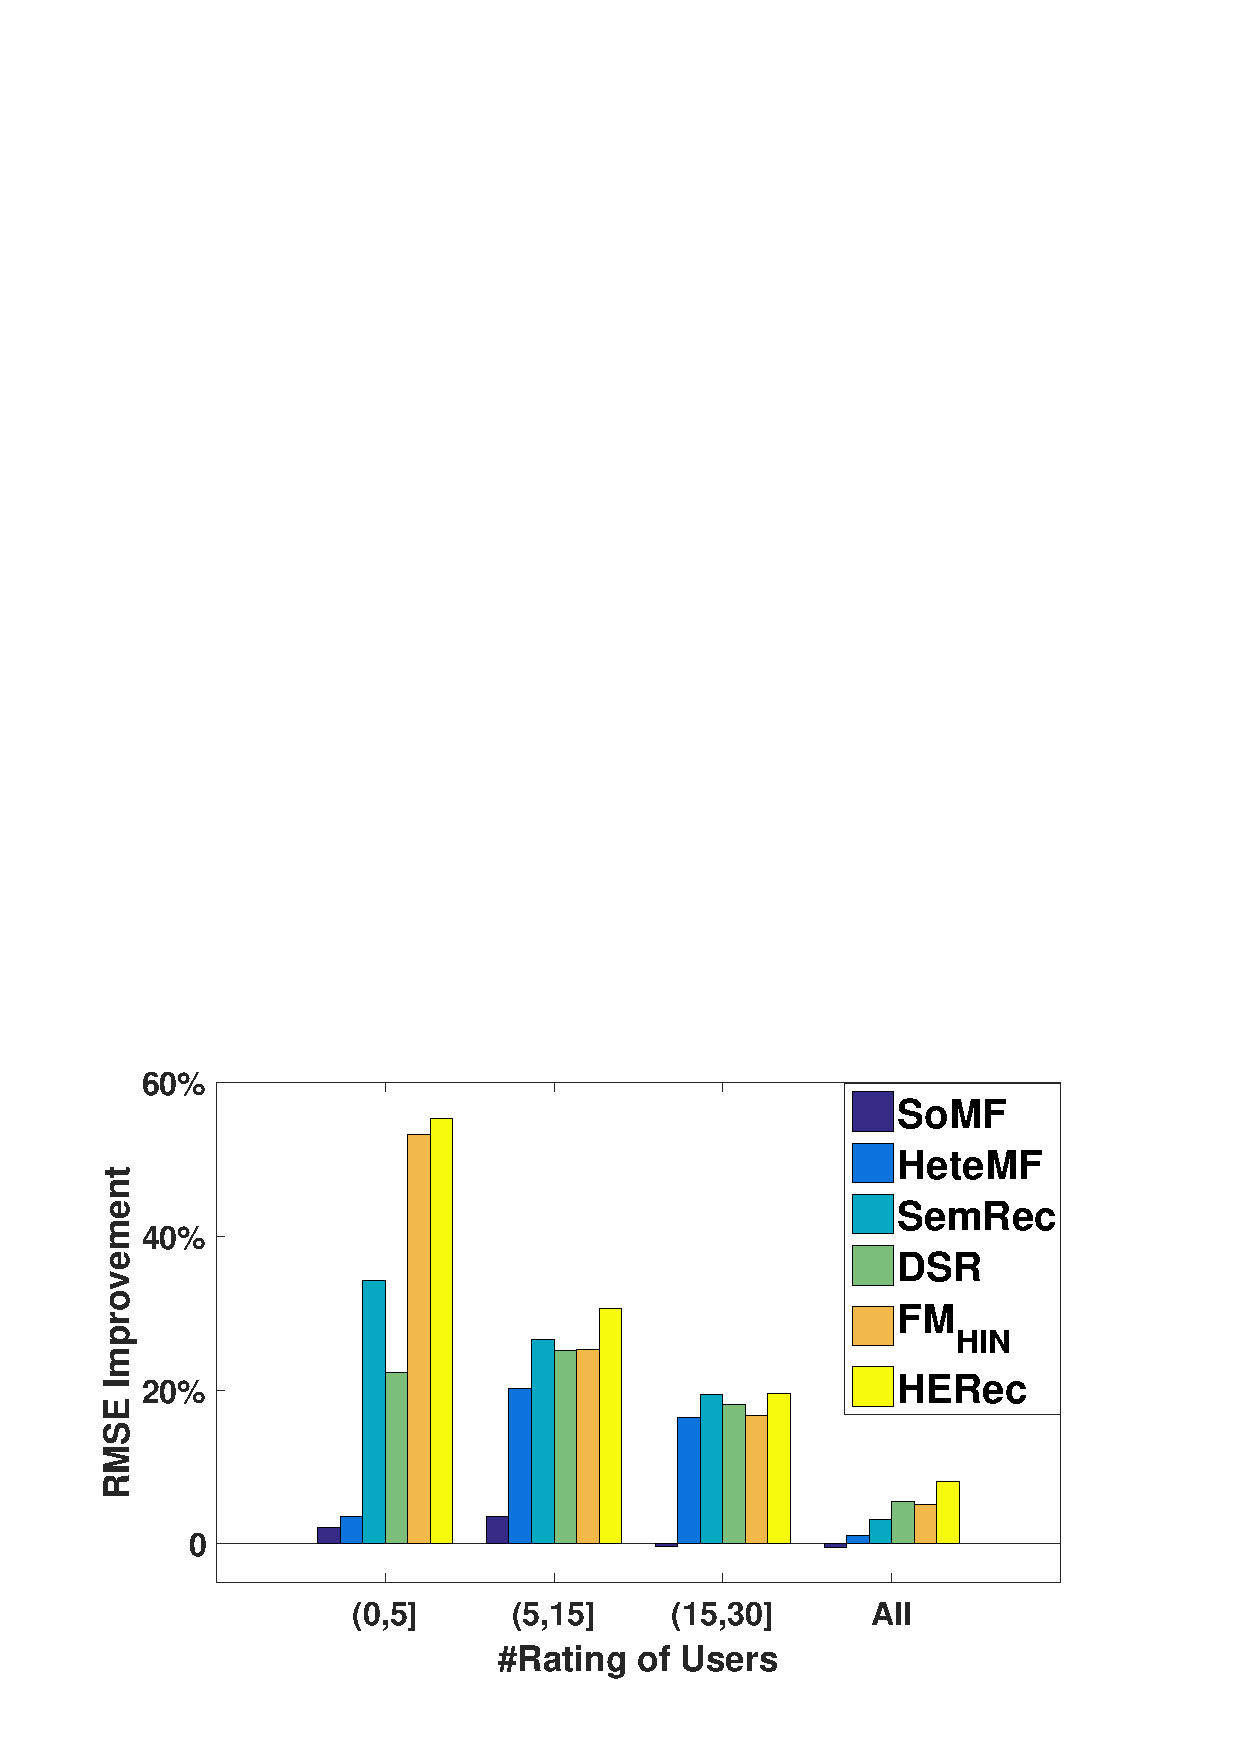
\includegraphics[width=4.2cm]{image/cold_start_rmse.pdf}
%\end{minipage}
%}
%\hspace{30pt}
%\subfigure[MAE]{
%\begin{minipage}[t]{0.3\linewidth}
%\centering
%\includegraphics[width=4.2cm]{image/cold_start_mae.pdf}
%\end{minipage}
%}
%\caption{\label{fig_cs}Performance comparison of different methods for cold-start prediction. Improvement ratios over PMF are reported.}
%\end{figure}

%\begin{figure}[t]%[htbp]
%\centering
%\subfigure[RMSE]{
%\begin{minipage}[t]{0.3\linewidth}
%\centering
%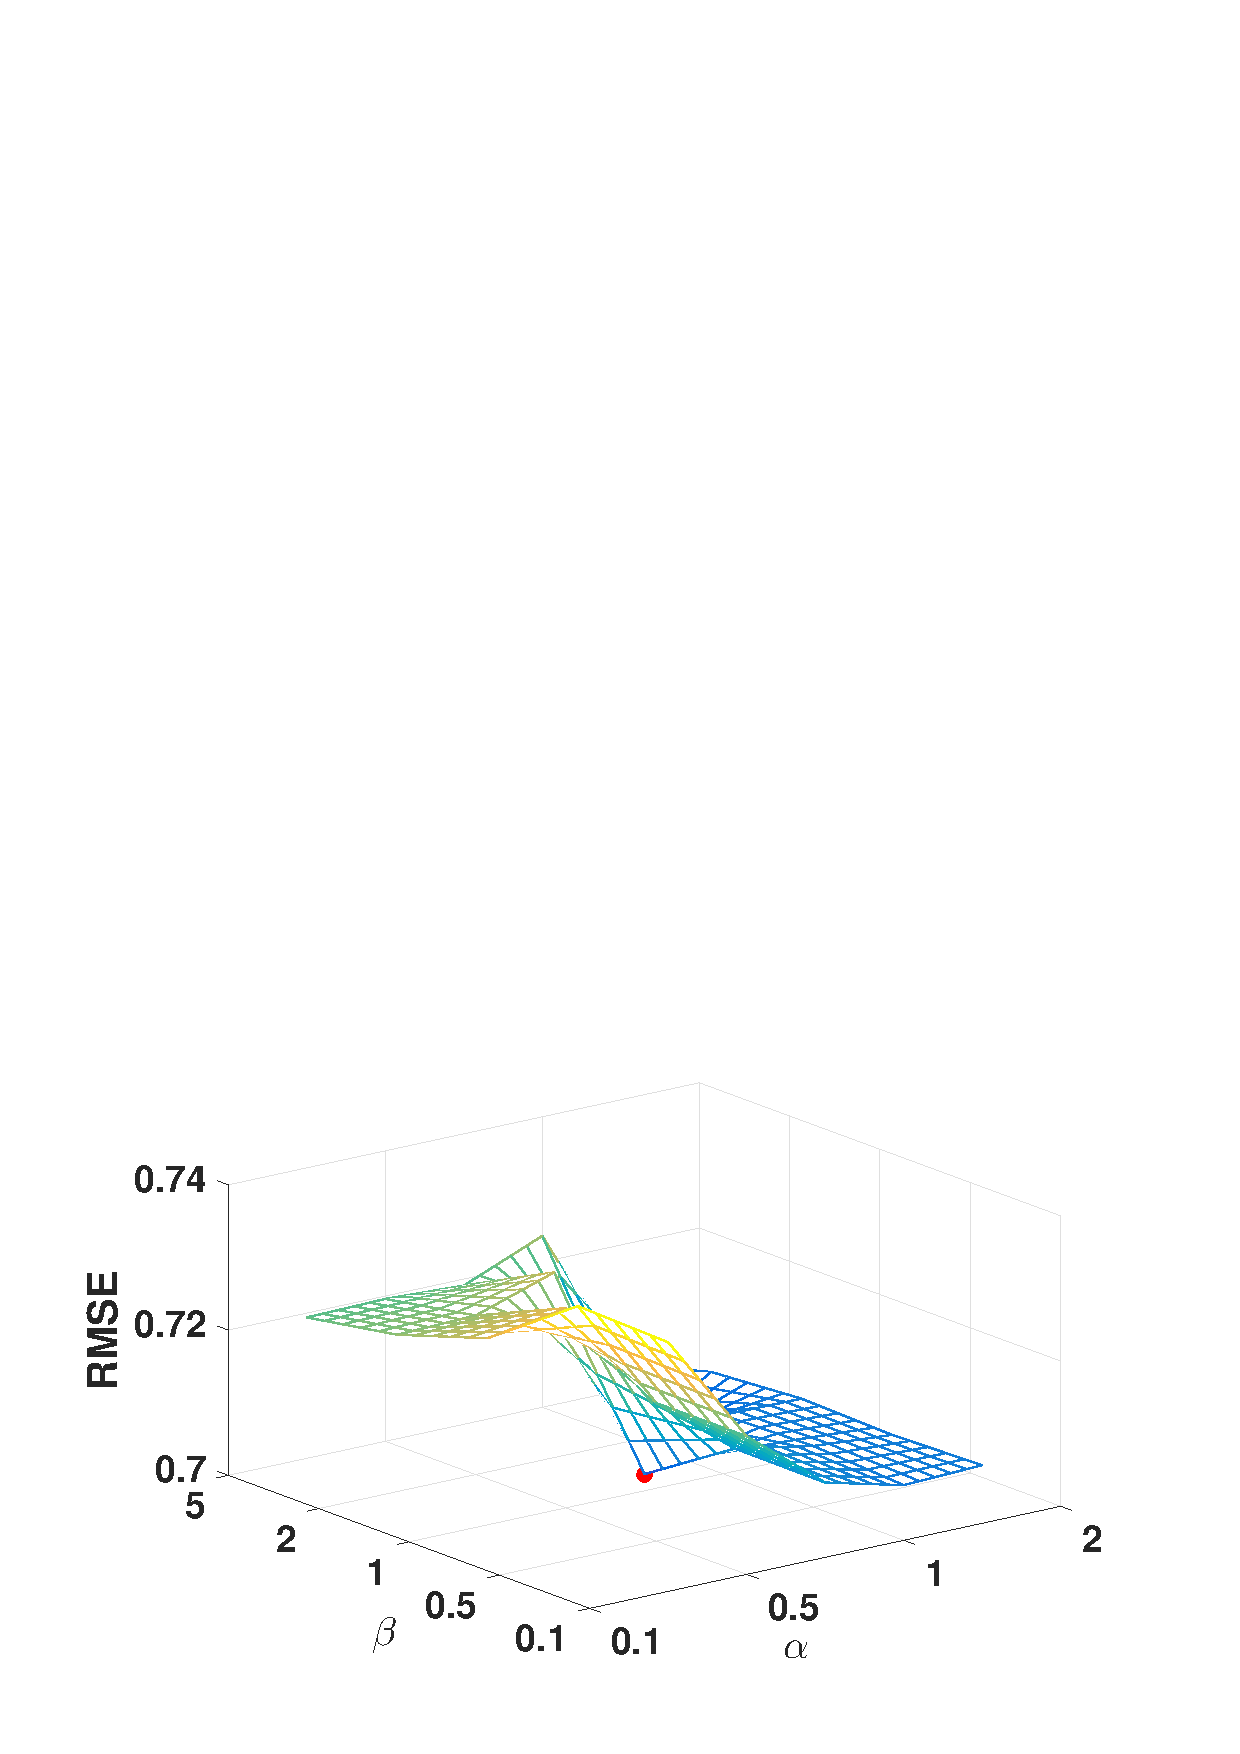
\includegraphics[width=4.2cm]{image/reg_rmse.pdf}
%\end{minipage}
%}
%\hspace{40pt}
%\subfigure[MAE]{
%\begin{minipage}[t]{0.3\linewidth}
%\centering
%\includegraphics[width=4.2cm]{image/reg_mae.pdf}
%\end{minipage}
%}
%\caption{\label{fig_reg}Varying parameters $\alpha$ and $\beta$.}
%\end{figure}


\subsection{Detailed Analysis of The Proposed Approach}
In this part, we perform a series of detailed analysis for the proposed approach.

%\begin{figure}[t]%[htbp]
%\centering
%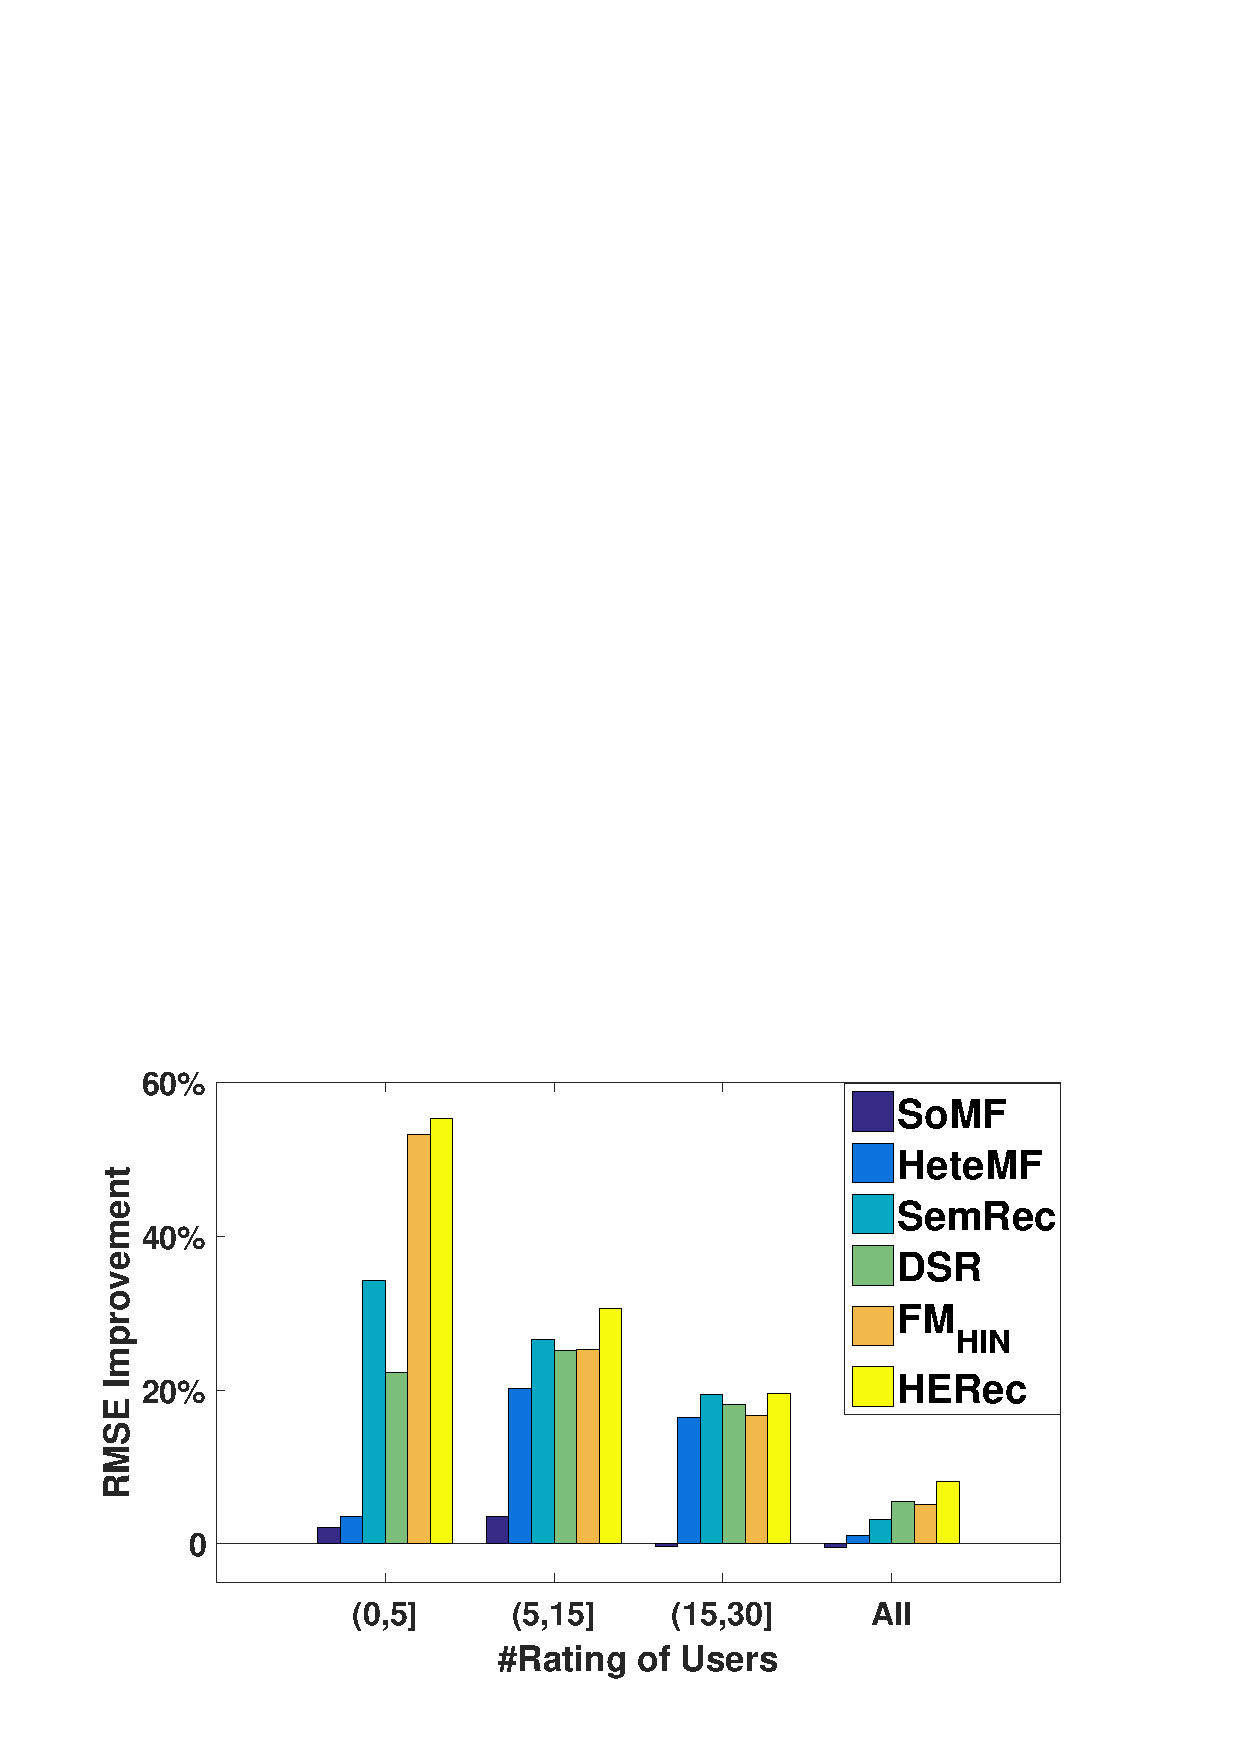
\includegraphics[width=8cm]{image/cold_start_rmse.pdf}
%\caption{\label{fig_cs}Performance comparison of different methods for cold-start prediction on Douban Movie dataset. $y$-axis denotes the improvement ratio over PMF.}
%\end{figure}

\begin{figure*}
\centering
\subfigure[Douban Movie]{
\begin{minipage}[b]{0.3\textwidth}
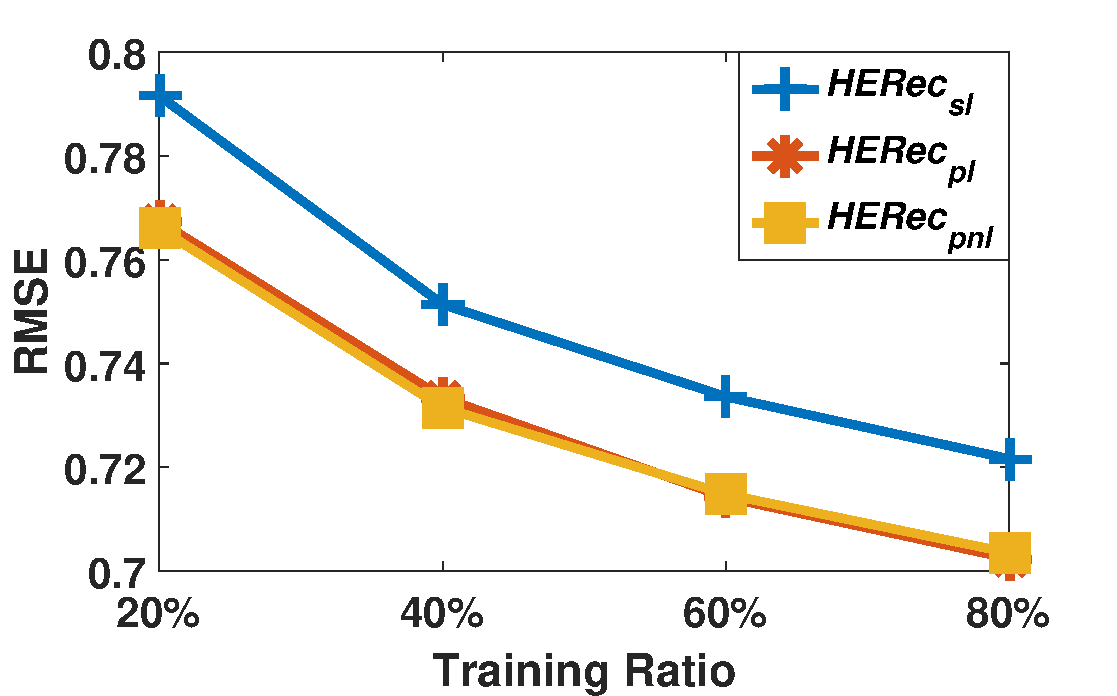
\includegraphics[width=1\textwidth]{image/fusion_dm_rmse.pdf} \\
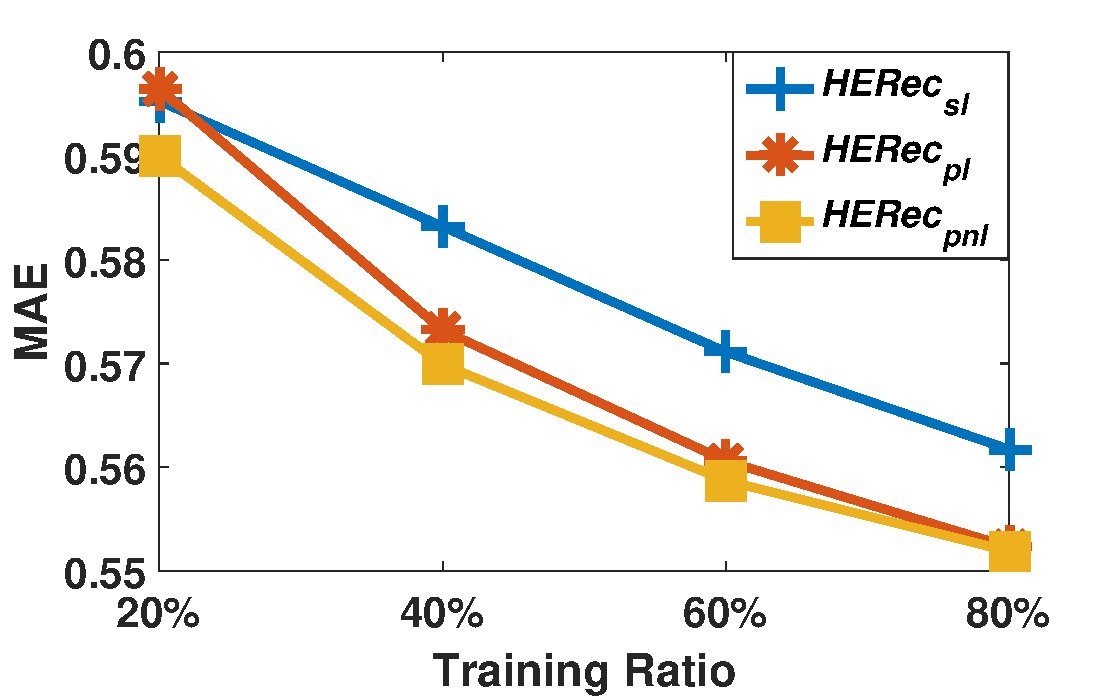
\includegraphics[width=1\textwidth]{image/fusion_dm_mae.pdf}
\end{minipage}
}
\subfigure[Douban Book]{
\begin{minipage}[b]{0.3\textwidth}
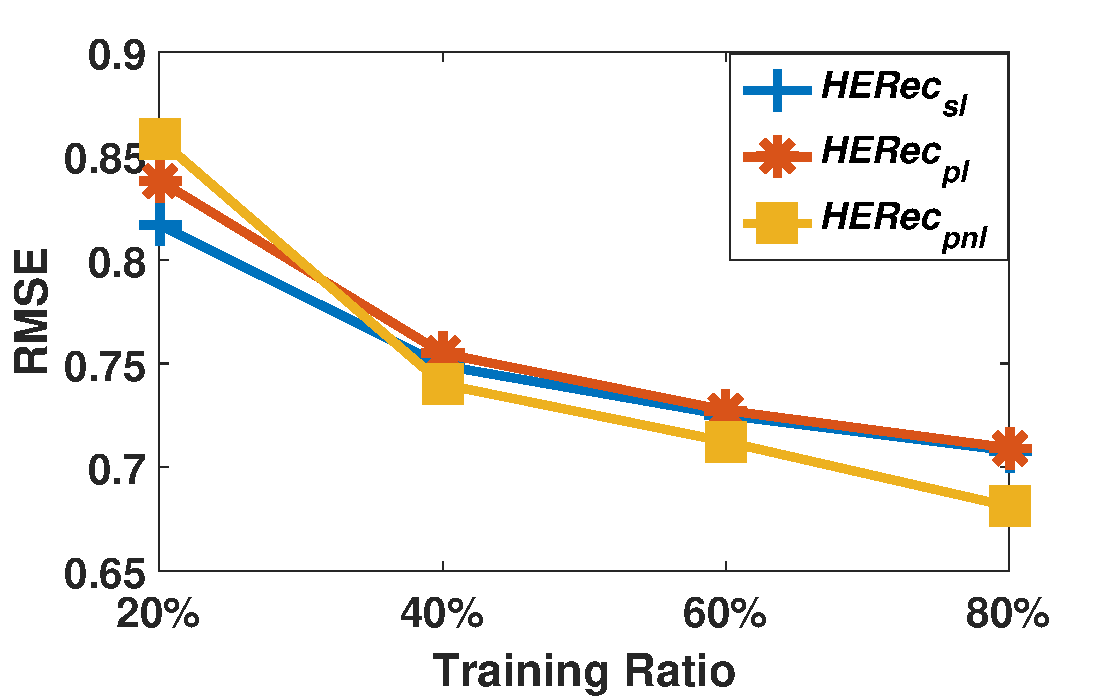
\includegraphics[width=1\textwidth]{image/fusion_db_rmse.pdf} \\
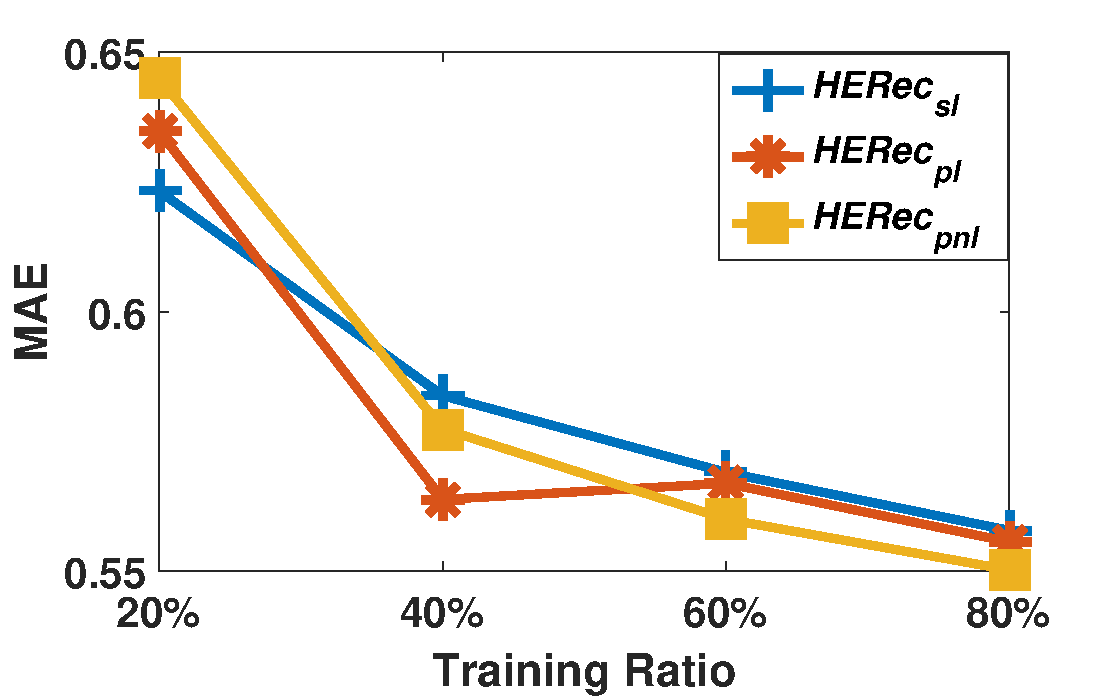
\includegraphics[width=1\textwidth]{image/fusion_db_mae.pdf}
\end{minipage}
}
\subfigure[Yelp]{
\begin{minipage}[b]{0.3\textwidth}
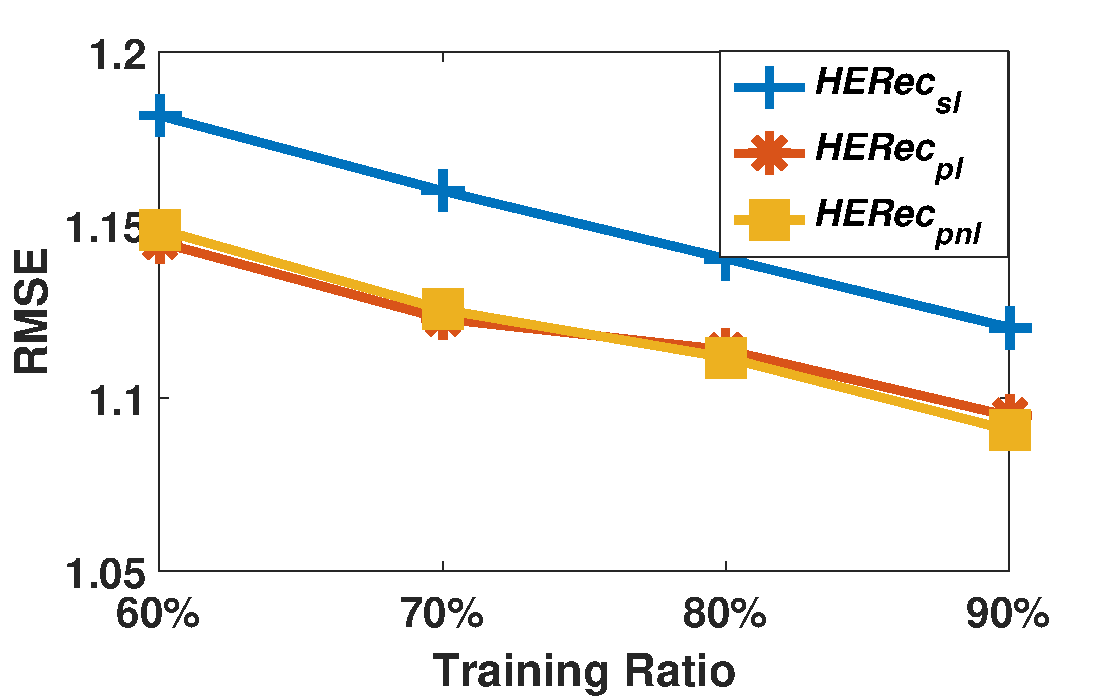
\includegraphics[width=1\textwidth]{image/fusion_yelp_rmse.pdf} \\
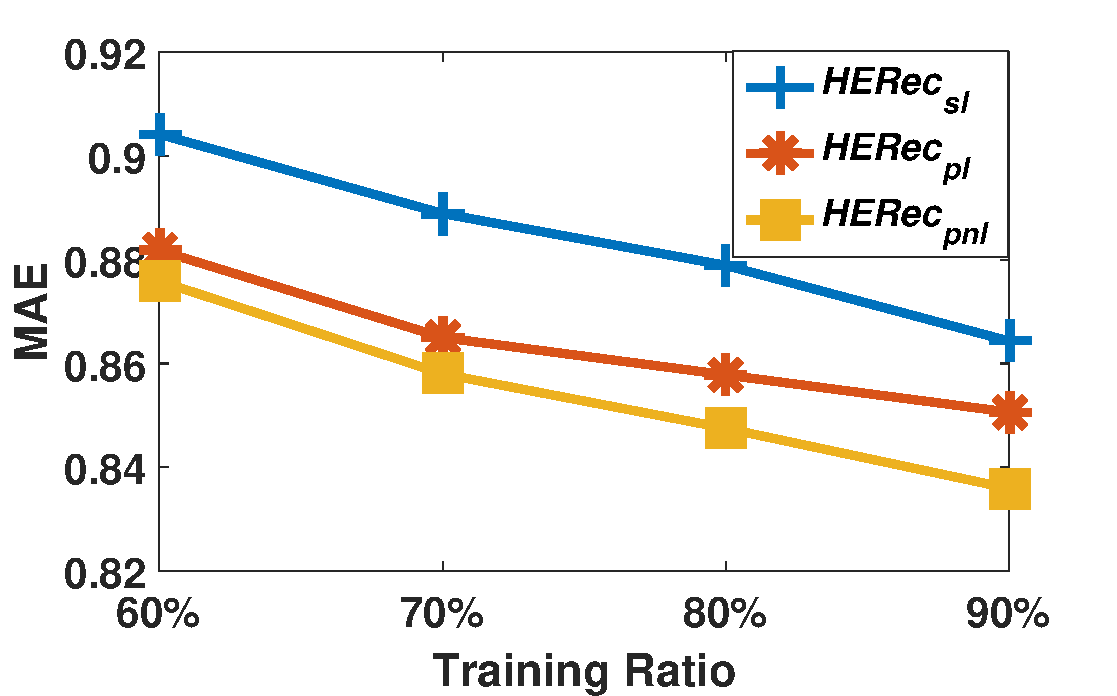
\includegraphics[width=1\textwidth]{image/fusion_yelp_mae.pdf}
\end{minipage}
}
\caption{\label{fig_fusion}Performance comparison of different fusion functions on three datasets.}
\end{figure*}

\begin{figure*}
\centering
\subfigure[Douban Movie]{
\begin{minipage}[b]{0.3\textwidth}
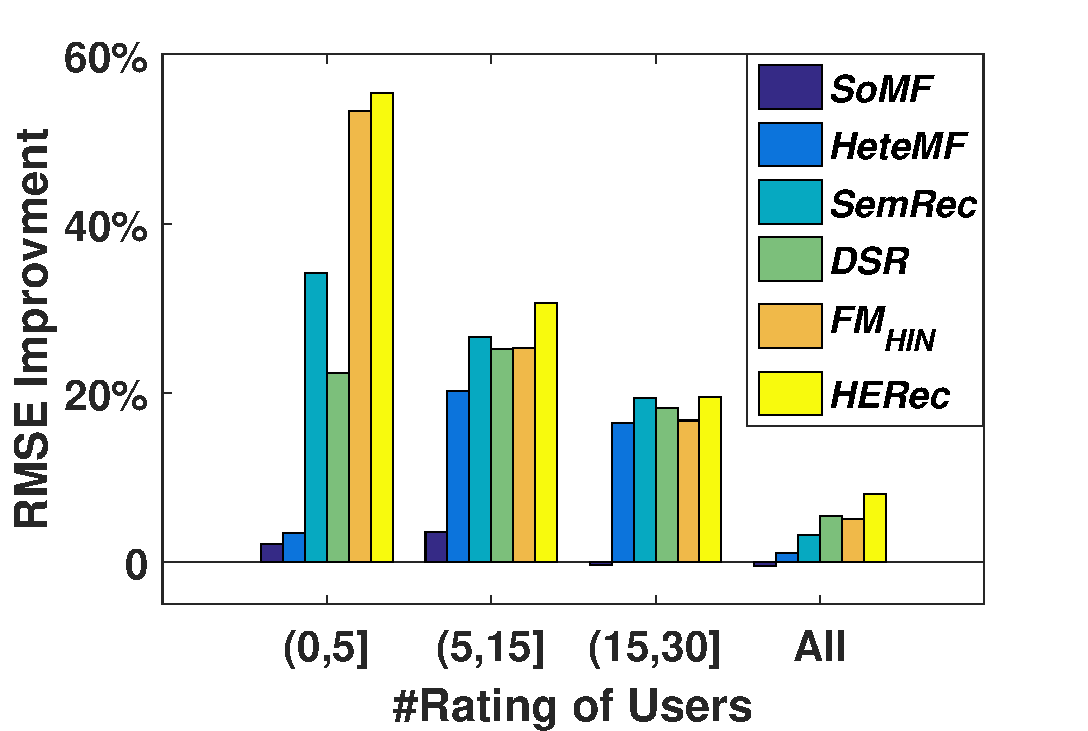
\includegraphics[width=1\textwidth]{image/cold_start_rmse_dm.pdf} \\
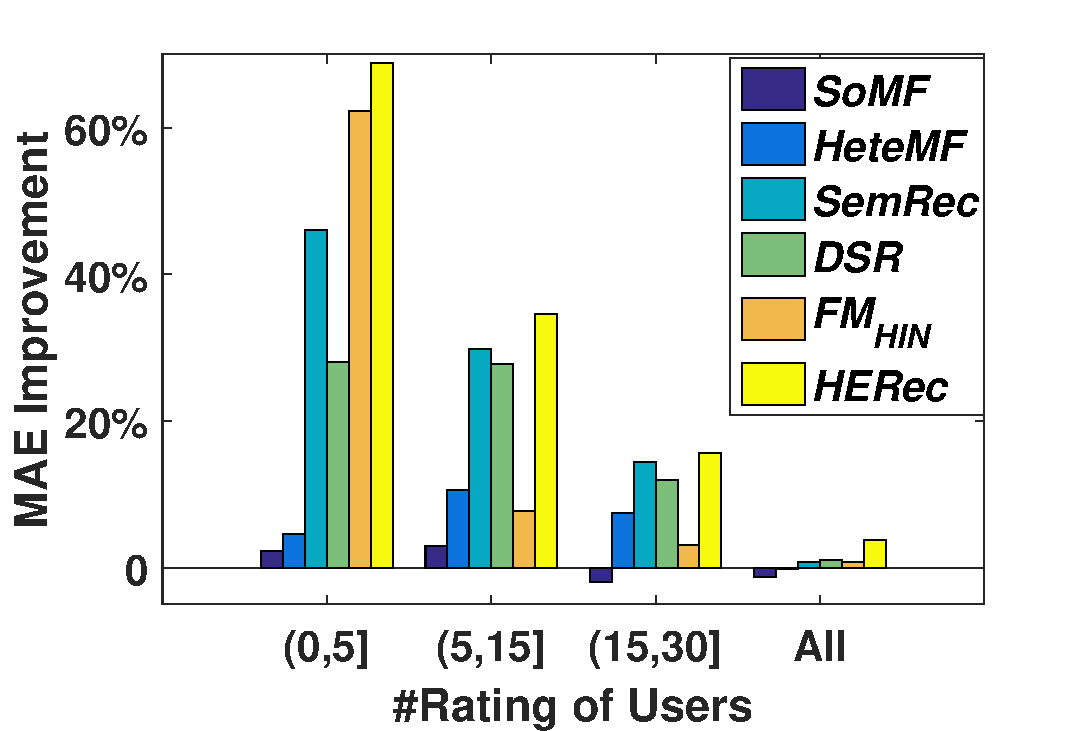
\includegraphics[width=1\textwidth]{image/cold_start_mae_dm.pdf}
\end{minipage}
}
\subfigure[Douban Book]{
\begin{minipage}[b]{0.3\textwidth}
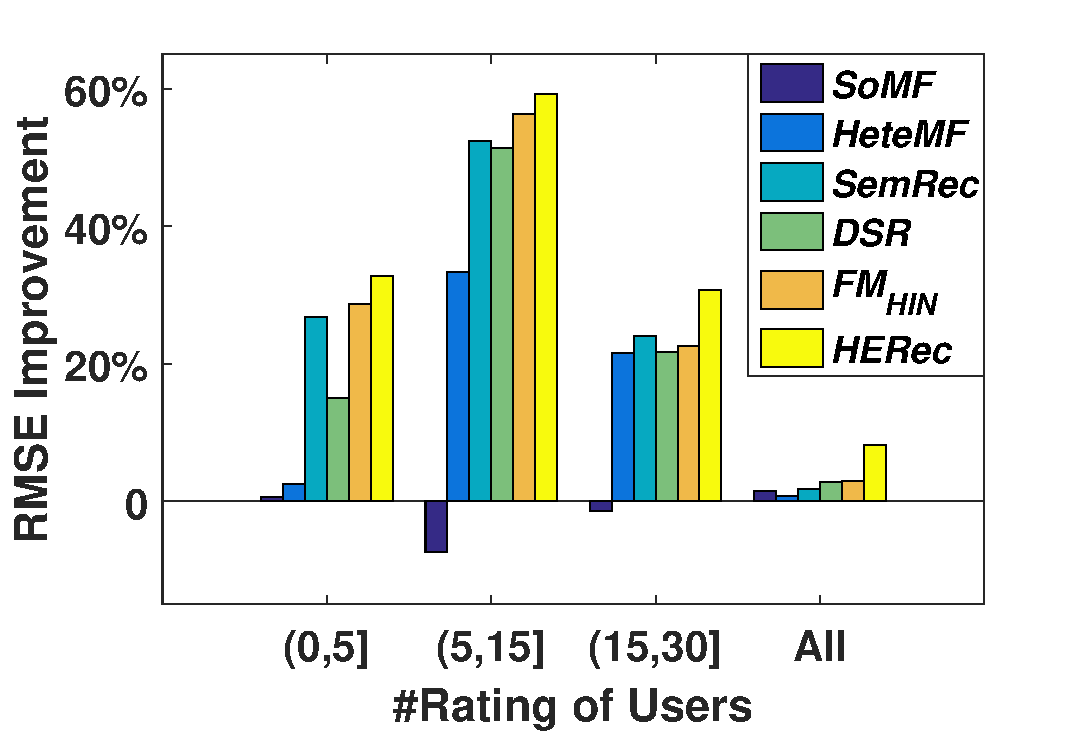
\includegraphics[width=1\textwidth]{image/cold_start_rmse_db.pdf} \\
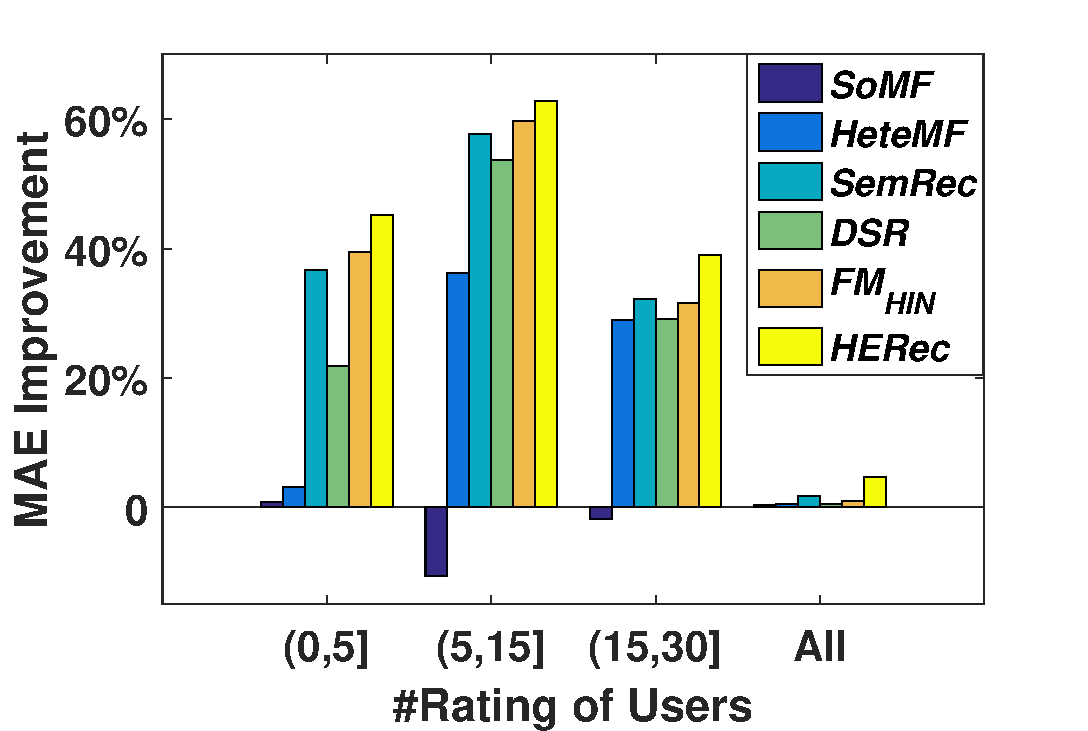
\includegraphics[width=1\textwidth]{image/cold_start_mae_db.pdf}
\end{minipage}
}
\subfigure[Yelp]{
\begin{minipage}[b]{0.3\textwidth}
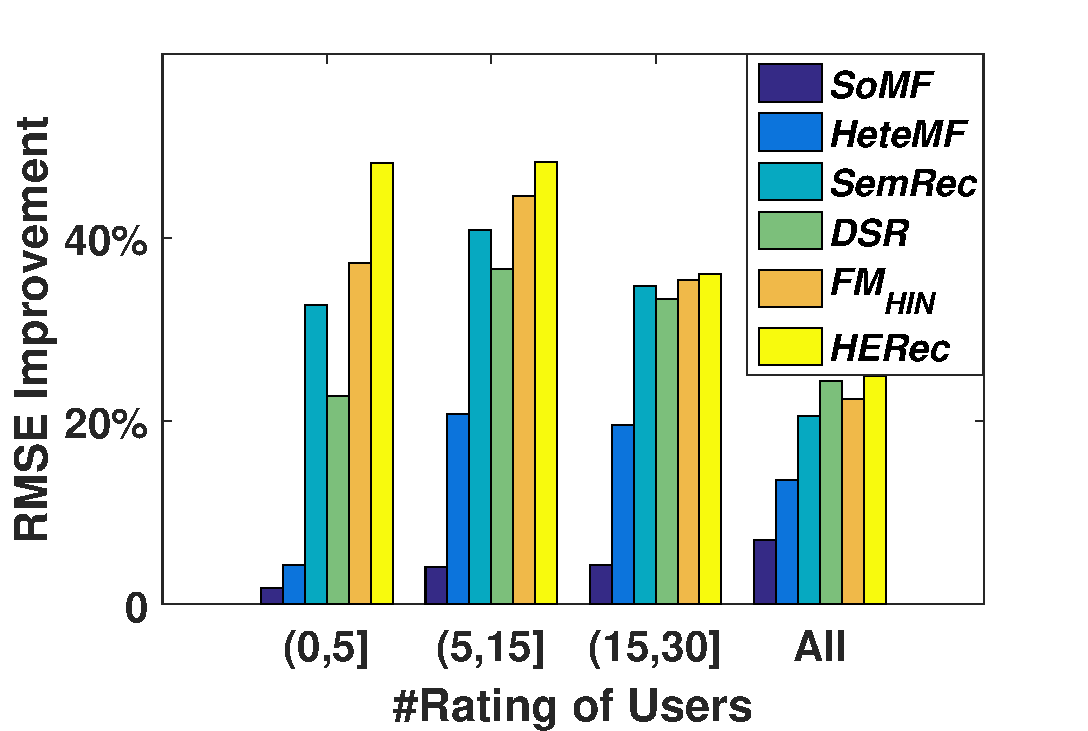
\includegraphics[width=1\textwidth]{image/cold_start_rmse_yelp.pdf} \\
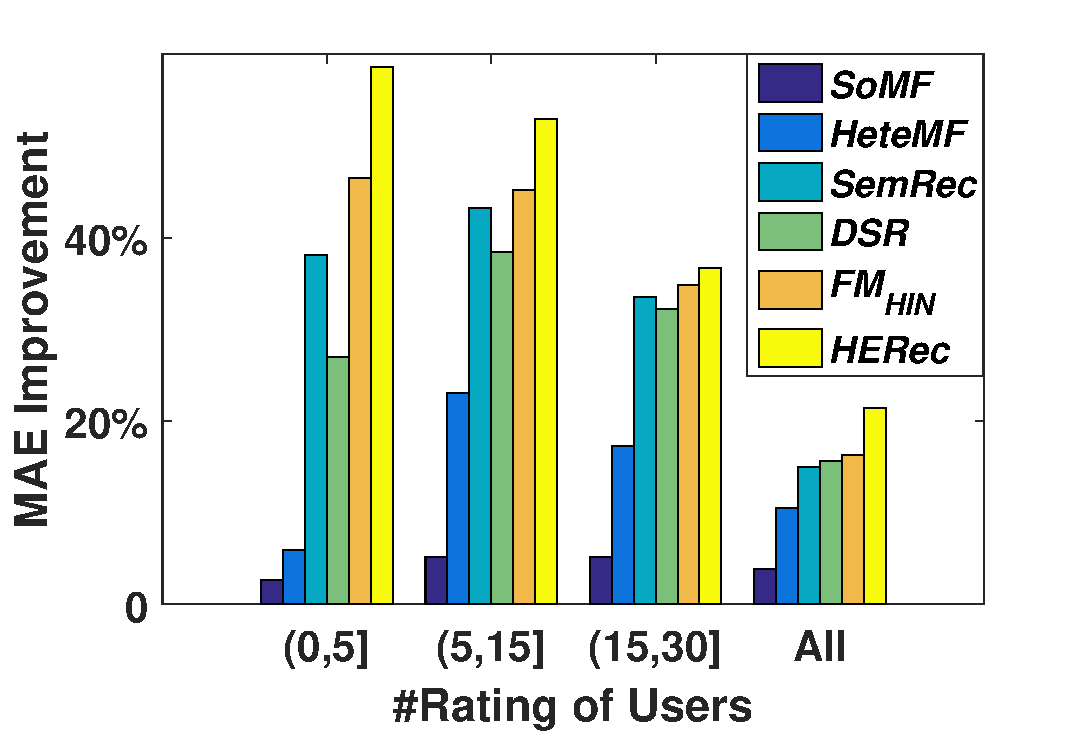
\includegraphics[width=1\textwidth]{image/cold_start_mae_yelp.pdf}
\end{minipage}
}
\caption{\label{fig_cs}Performance comparison of different methods for cold-start prediction on three datasets. $y$-axis denotes the improvement ratio over PMF.}
\end{figure*}

\subsubsection{Selection of Different Fusion Functions}
HERec requires a principled fusion way to transform node embeddings into a more suitable form that is useful to enhance recommendation performance. Therefore, we will discuss the impact of different fusion functions on the recommendation performance.
For convenience, we call the HERec variant with the simple linear fusion function (Eq.~\ref{eq-slf}) as HERec$_{sl}$, the variant with personalized linear fusion function  (Eq.~\ref{eq-plf}) as HERec$_{pl}$,  and the variant with personalized non-linear fusion function (Eq.~\ref{eq-pnlf}) as HERec$_{pnl}$.
We present the performance comparison of the three variants of HERec on the three datasets in Fig.~\ref{fig_fusion}.

As shown in Fig.~\ref{fig_fusion}, we can find that overall performance ranking is as follows: HERec$_{pnl}$ $>$ HERec$_{pl}$ $>$ HERec$_{sl}$. Among the three variants, the simple linear fusion function performs the worst, as it ignores the personalization and non-linearity. Indeed, users are likely to have varying preferences over meta-paths~\cite{shi2015semantic}, which should be considered in meta-path based methods. The personalization factor improves the performance significantly. As a comparison, the performance improvement of
HERec$_{pnl}$ over  HERec$_{pl}$ is relatively small. A possible reason is that the incorporation of personalized combination parameters increases the capability of linear models. Nonetheless, HERec$_{pnl}$ still performs the best by considering personalization and non-linear transformation.
In a complicated recommender setting, HIN embeddings may not be directly applicable in recommender systems, where a non-linear mapping function is preferred.

Since HERec$_{pnl}$ is the best variant of the proposed model, in what follows, HERec will use the personalized non-linear fusion function, \ie HERec$_{pnl}$ by default.

\subsubsection{Cold-start Prediction}
HINs are particularly useful to improve cold-start prediction, where there are fewer rating records but heterogeneous context information is available. We consider studying the performance \emph{w.r.t.} different cold-start degrees, \ie the rating sparsity.
To test it, we first  categorize ``cold" users into three groups according to the numbers of their rating records, \ie $(0, 5]$, $(5, 15]$ and $(15, 30]$. It is easy to see that the case for the first group is the most difficult, since users from this group have fewest rating records.
Here, we only select the baselines which use HIN based information for recommendation, including SoMF, HeteMF, SemRec, DSR and FM$_{HIN}$.
We present the performance comparison of different methods in Fig.~\ref{fig_cs}. For convenience, we report the improvement ratios \emph{w.r.t.} PMF.
Overall, all the comparison methods are better than PMF (\ie a positive $y$-axis value). The proposed method performs the best among all the methods, and the improvement over PMF becomes more significant for users with fewer rating records. The results indicate that HIN based information is effective to improve the recommendation performance, and the proposed HERec method can effectively utilize HIN information in a more principled way.



%\begin{figure}[htbp]
%%\centering
%\subfigure[Yelp]{
%\begin{minipage}[t]{0.3\linewidth}
%\centering
%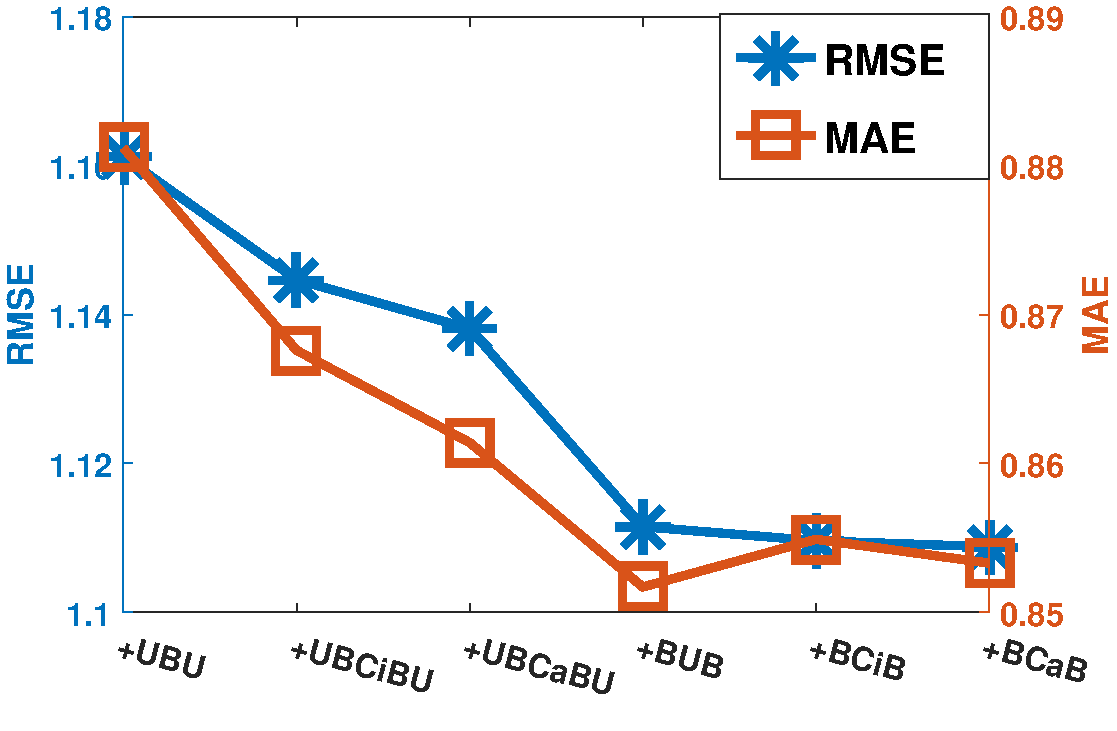
\includegraphics[width=4.2cm]{image/metapath_yelp.pdf}
%\end{minipage}
%}
%\hspace{40pt}
%\subfigure[Douban Movie]{
%\begin{minipage}[t]{0.3\linewidth}
%\centering
%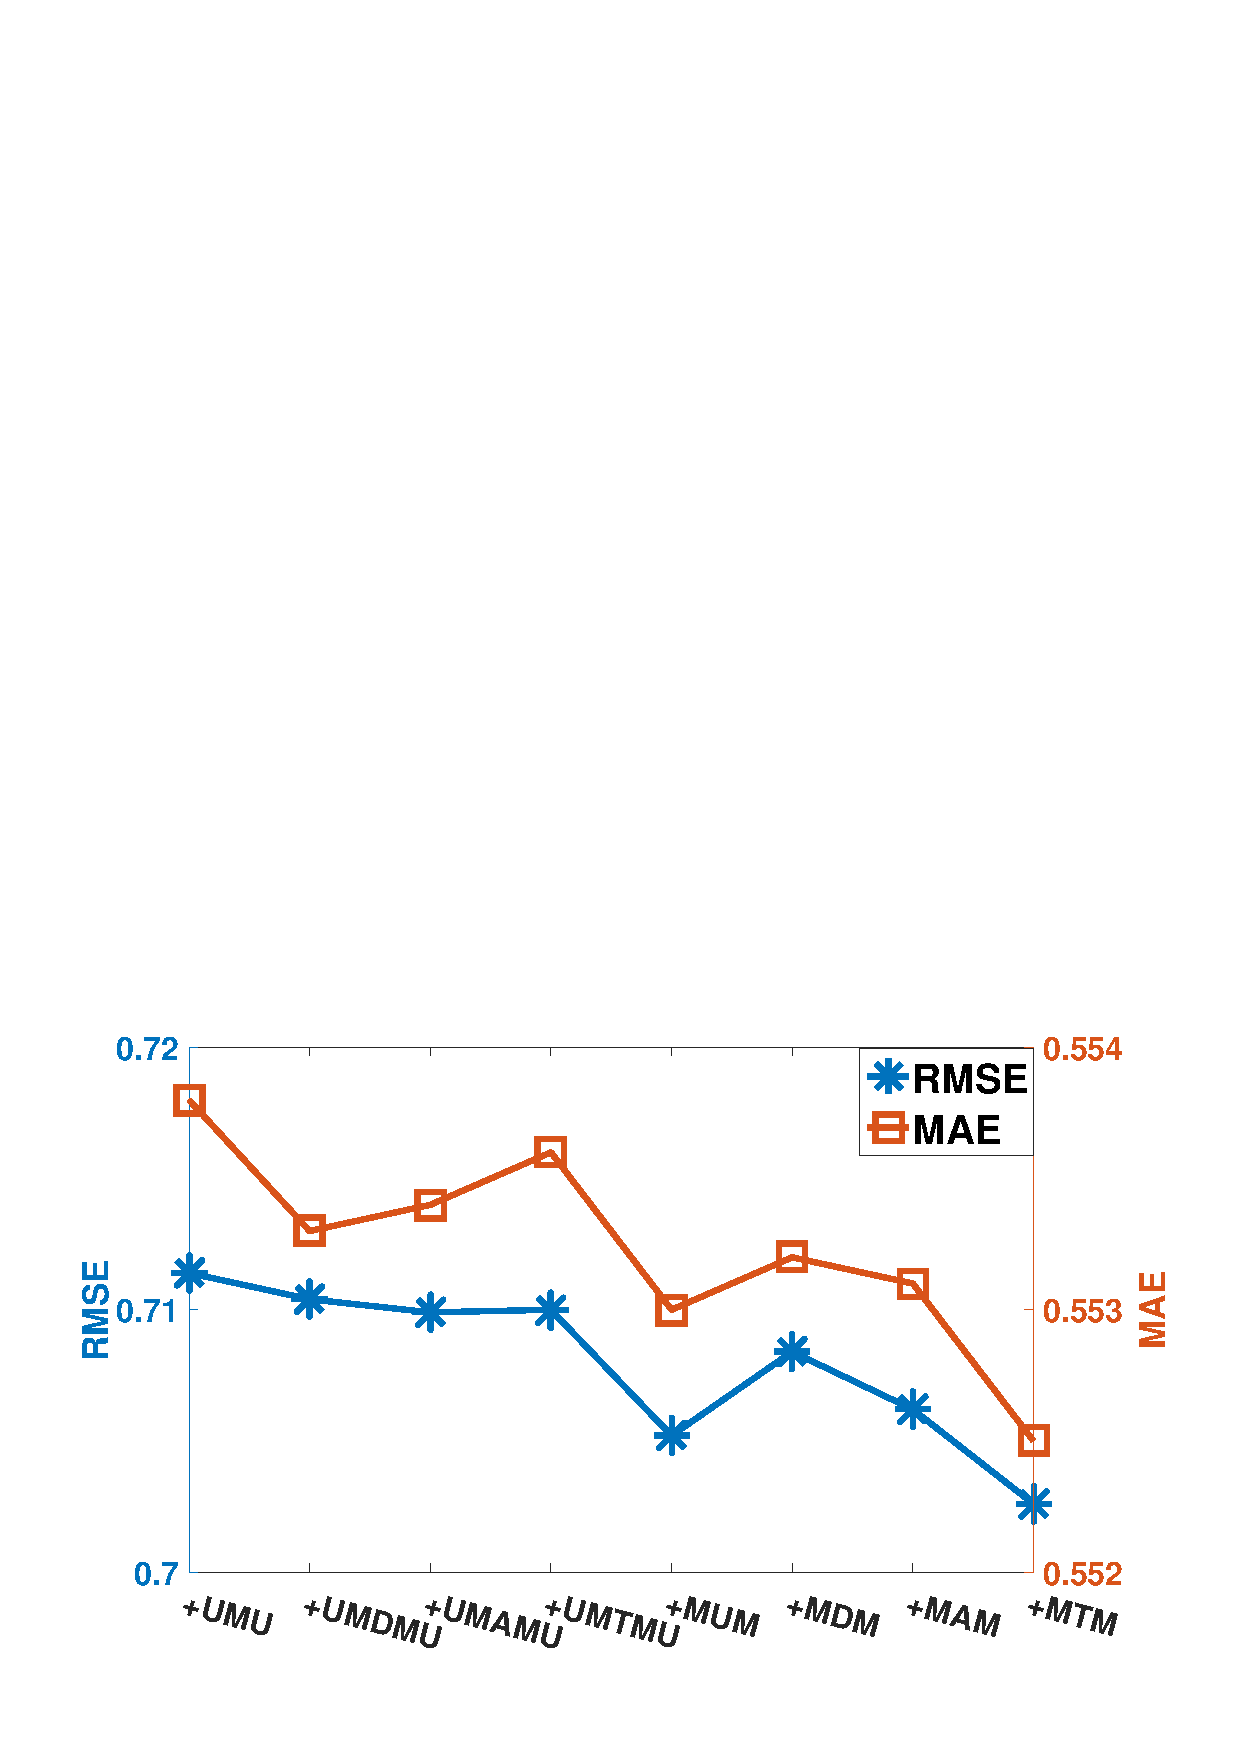
\includegraphics[width=4.2cm]{image/metapath_douban.pdf}
%\end{minipage}
%}
%\caption{\label{fig_metapath}Performance change of HERec when gradually incorporating meta-paths.}
%\end{figure}

%\begin{figure}[htbp]
%%\centering
%\subfigure[Yelp]{
%\begin{minipage}[t]{0.5\textwidth}
%\centering
%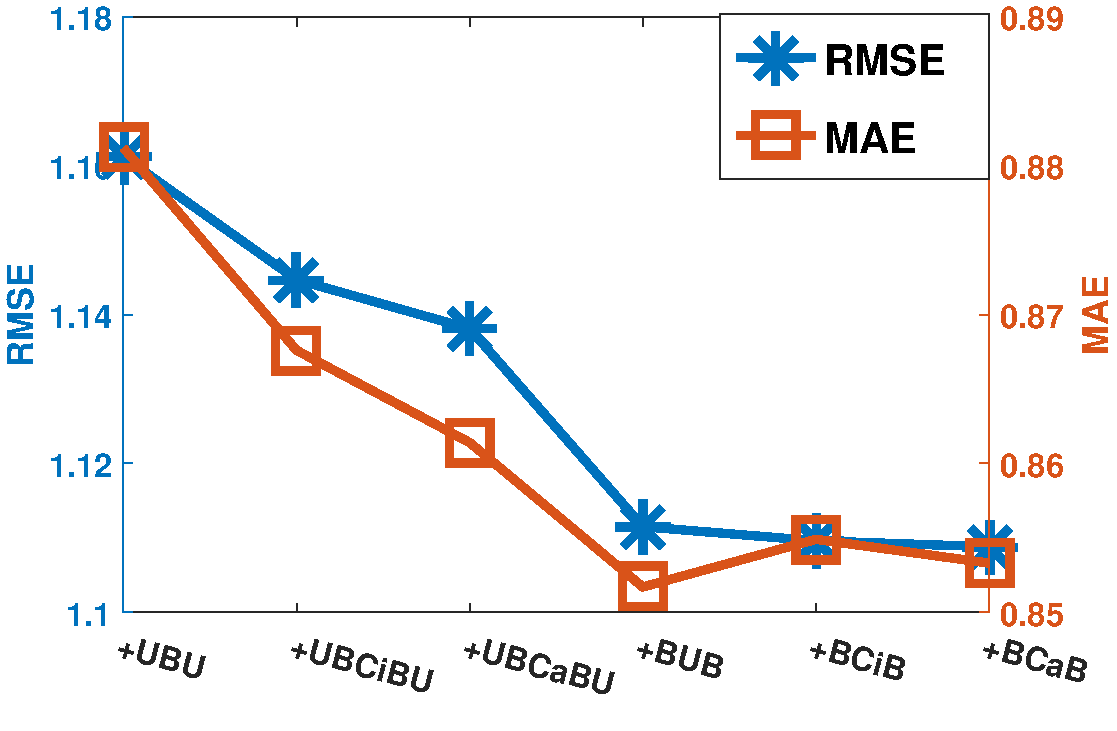
\includegraphics[width=8cm]{image/metapath_yelp.pdf}
%\end{minipage}
%}
%\subfigure[Douban Movie]{
%\begin{minipage}[t]{0.5\textwidth}
%\centering
%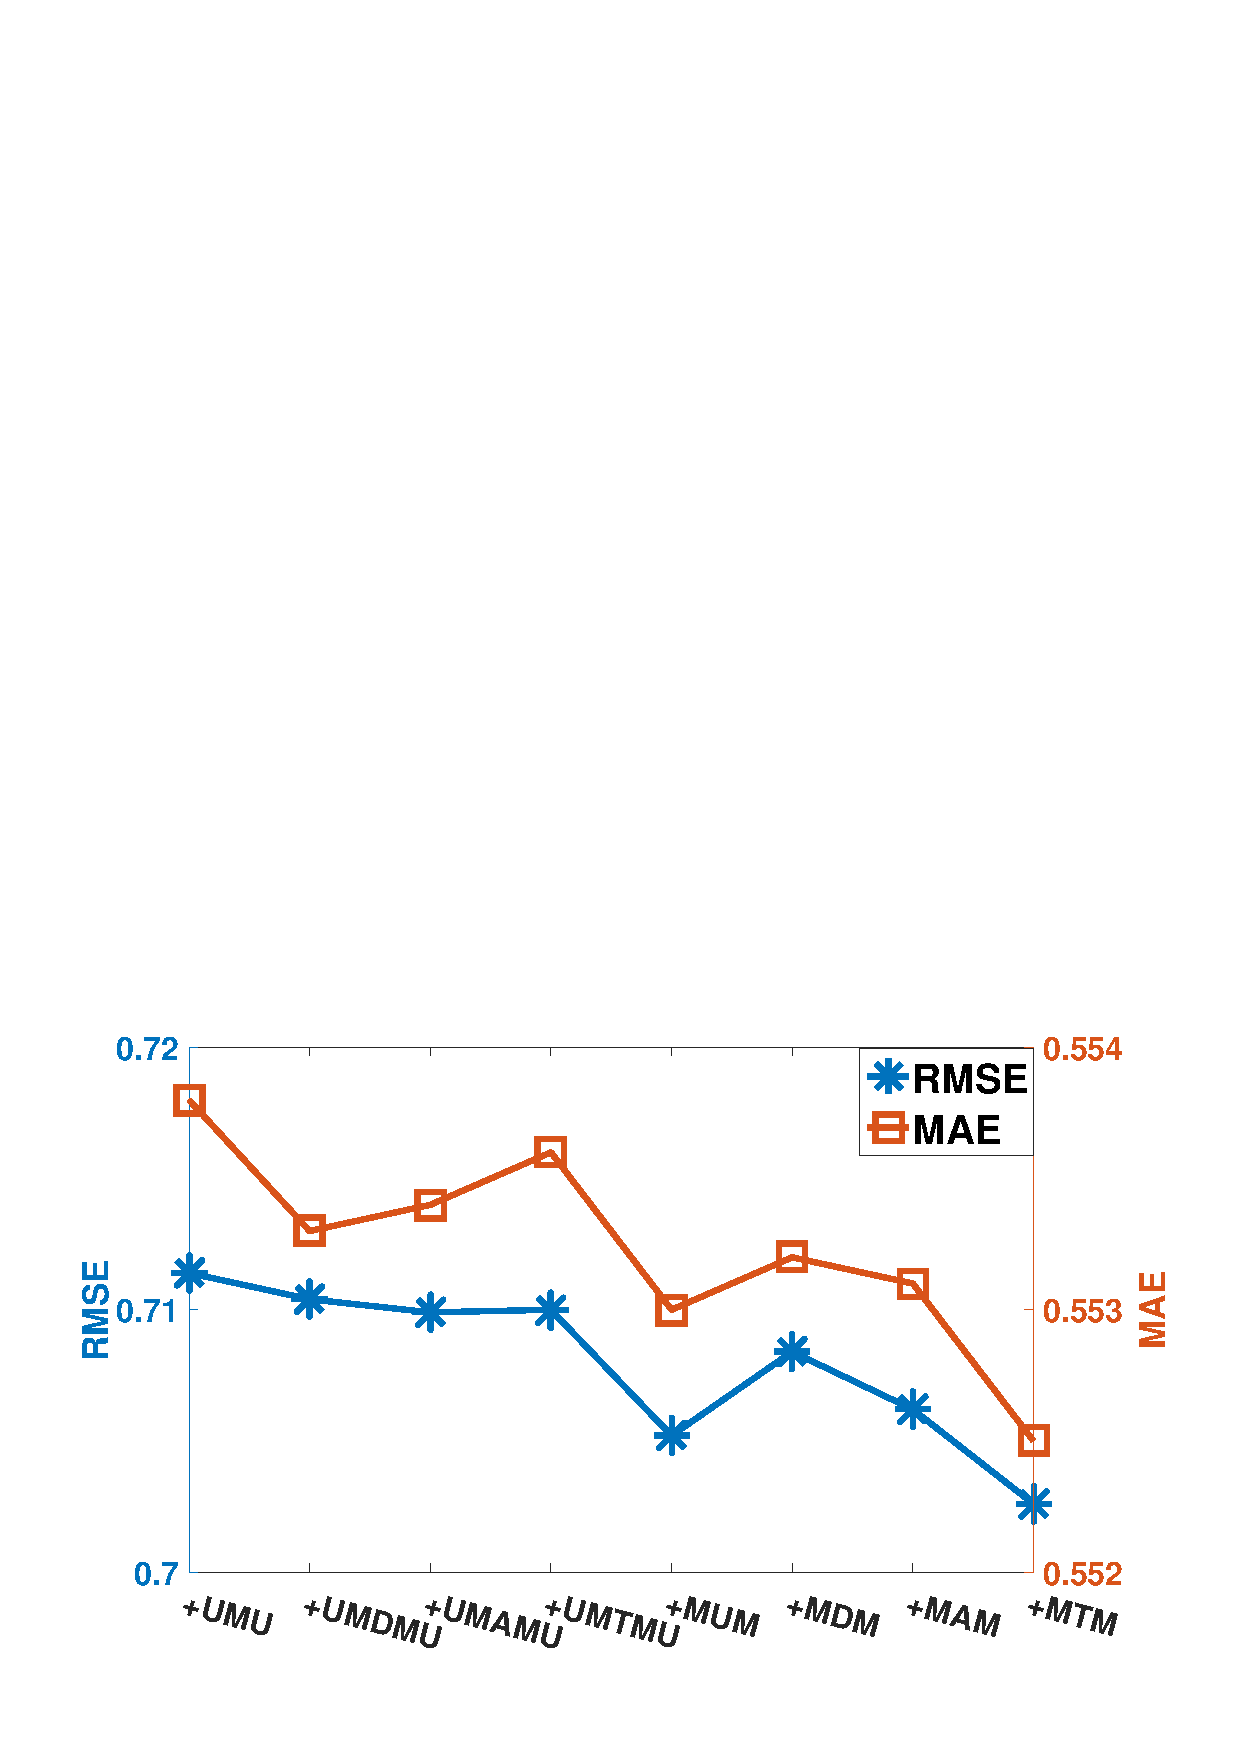
\includegraphics[width=8cm]{image/metapath_douban.pdf}
%\end{minipage}
%}
%\caption{\label{fig_metapath}Performance change of HERec when gradually incorporating meta-paths.}
%\end{figure}

\begin{figure*}[htbp]
\centering
\subfigure[Douban Movie]{
\begin{minipage}[t]{0.3\textwidth}
\centering
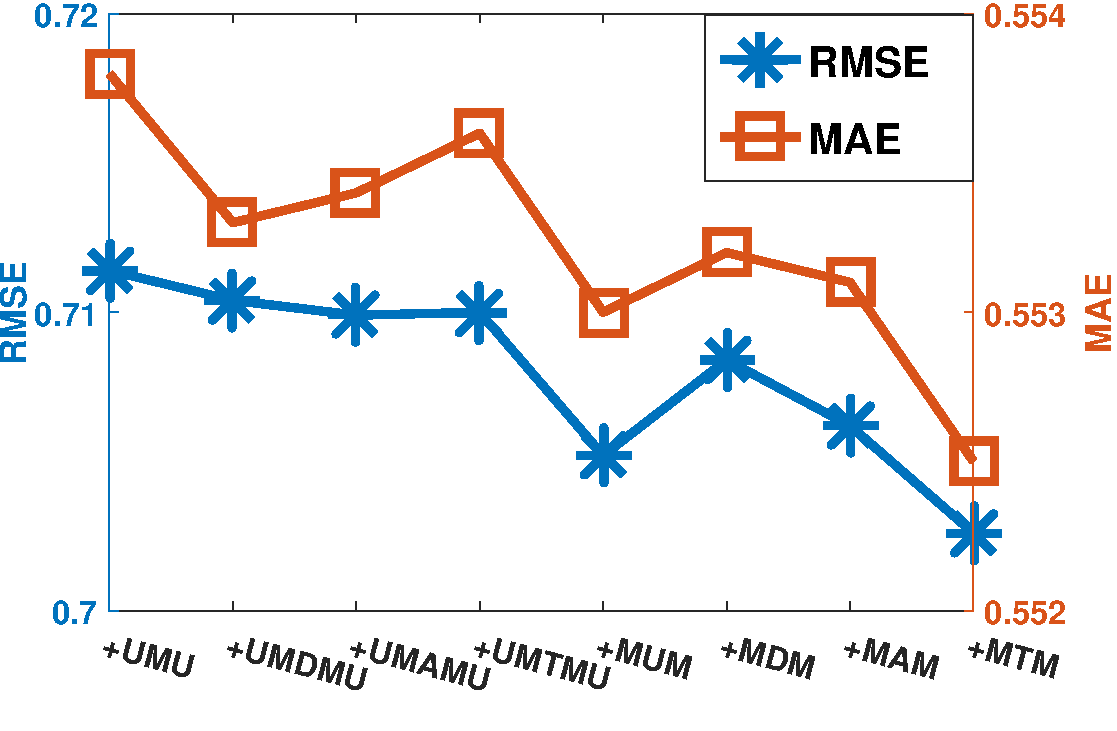
\includegraphics[width=1\textwidth]{image/metapath_dm.pdf}
\end{minipage}
}
\subfigure[Douban Book]{
\begin{minipage}[t]{0.3\textwidth}
\centering
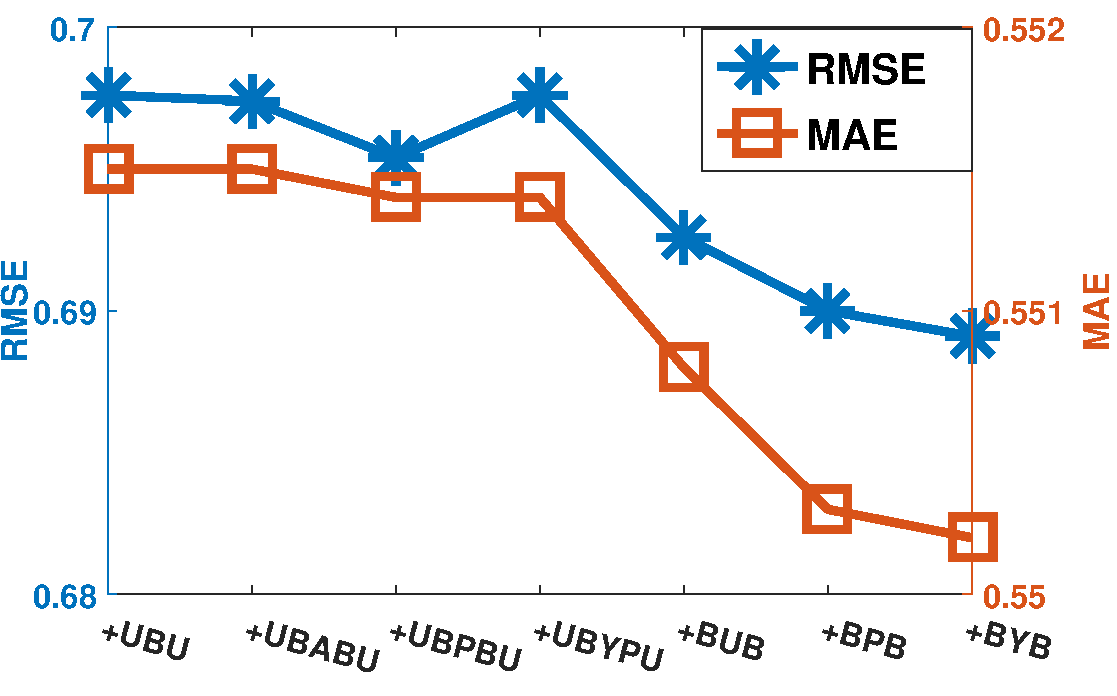
\includegraphics[width=1.05\textwidth]{image/metapath_db.pdf}
\end{minipage}
}
\subfigure[Yelp]{
\begin{minipage}[t]{0.3\textwidth}
\centering
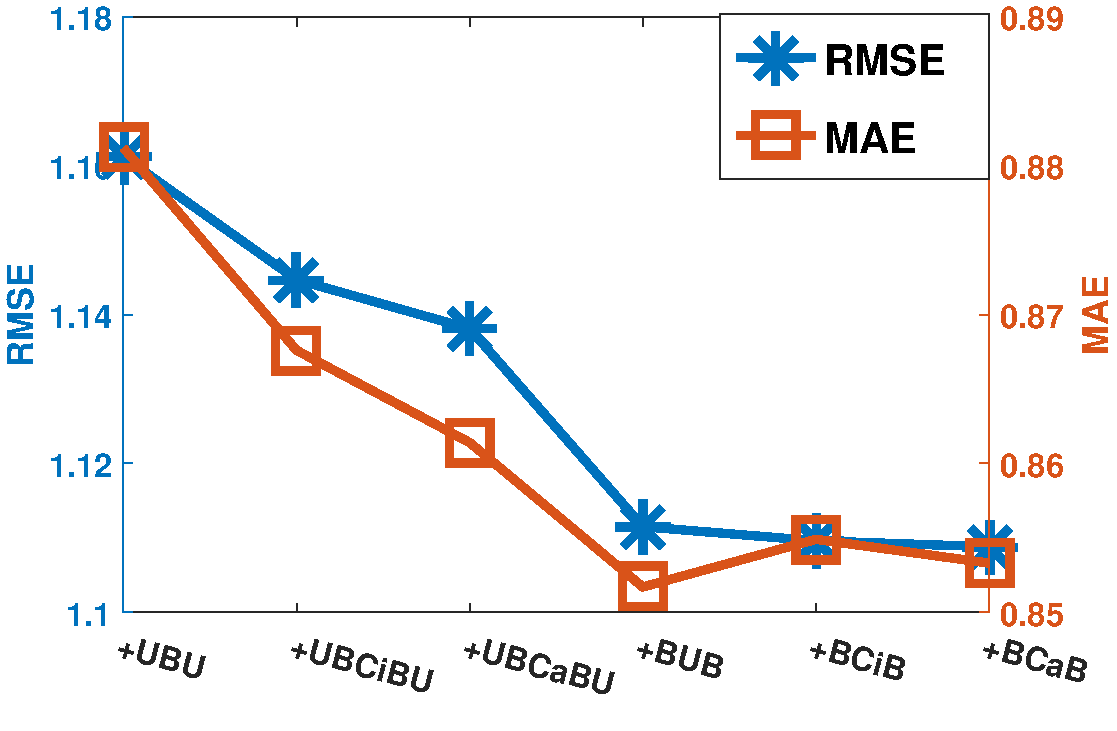
\includegraphics[width=1\textwidth]{image/metapath_yelp.pdf}
\end{minipage}
}
\caption{\label{fig_metapath}Performance change of HERec when gradually incorporating meta-paths.}
\end{figure*}



\subsubsection{Impact of Different Meta-Paths}
%Our approach depends on the selection of useful meta-paths.
As shown in Table~\ref{tab_Data}, the proposed approach uses a selected set of meta-paths.
To further analyze the impact of different meta-paths, we gradually incorporate these meta-paths into the proposed approach and check the performance change.
In Fig. \ref{fig_metapath}, we can observe that generally the performance improves (\ie becoming smaller) with the incorporation of more meta-paths.
Both meta-paths starting with the user type and item type are useful to improve the performance.
However, it does not always yield the improvement with more meta-paths, and the performance slightly fluctuates.
The reason is that some meta-paths may contain noisy  or conflict information with existing ones.
Another useful observation is that the performance quickly achieves a relatively good performance with the incorporation of only a few meta-paths.
This confirms previous finding~\cite{shi2015semantic}:  a small number of high-quality meta-paths are able to lead to large performance improvement. Hence, as mentioned before, we can effectively control the model complexity by selecting just a few meta-paths.

%As mentioned before, this finding is implicative
%Our approach converts the meta-path information into embeddings subsequently transformed by a learnable function, which is able to reduce the noisy influence from meta-paths to some extent.


%In this section, we study the impact of meta-paths on performances of HERec. We do experiments on Yelp and Douban Movie dataset via successively adding meta-paths to the HIN embedding phrase of HERec. The results are recorded in Fig. \ref{fig_metapath}. We can obverse that, with the addition of meta-paths, the HERec generally achieves better performances, which verifies that the multiple-perspective information extracted from multiple meta-paths is helpful to improve recommendation performance. Particularly, the performances are dramatically improved  when adding meta-paths of items (e.g., $BUB$ in Yelp and $MUM$ in Douban Movie), since it will integrate structure information of items into the model. On the other hand, we can also find that the recommendation performances are not always improved with the addition of more meta-paths, like the addition of $BCiB$ in Yelp and $MDM$ in Douban Movie. We think the reason lies in that, although meaningful meta-paths (e.g., $UBCiBU$ in Yelp and $UMDMU$ in Douban Movie) can provide valuable structural information for recommendation, while some meta-paths (e.g., $BCiB$ and $MDM$) have less valuable structural information but contain much noise information, which will harm the recommendation performance.
%Each meta path based embedding has different semantic information which would have different effects on recommendation performance. We notice the recommendation performance gains obviously significant improvement when add first several meta-paths. And when we continue adding meta-path, the improvement would be quite slight on RMSE, and even has the decreasing tendency on MAE. It verifies that meaningful mete-path would dramatically improve recommendation performance, while normal meta-path is helpless to recommendation.

%\begin{figure}[htbp]
%\centering
%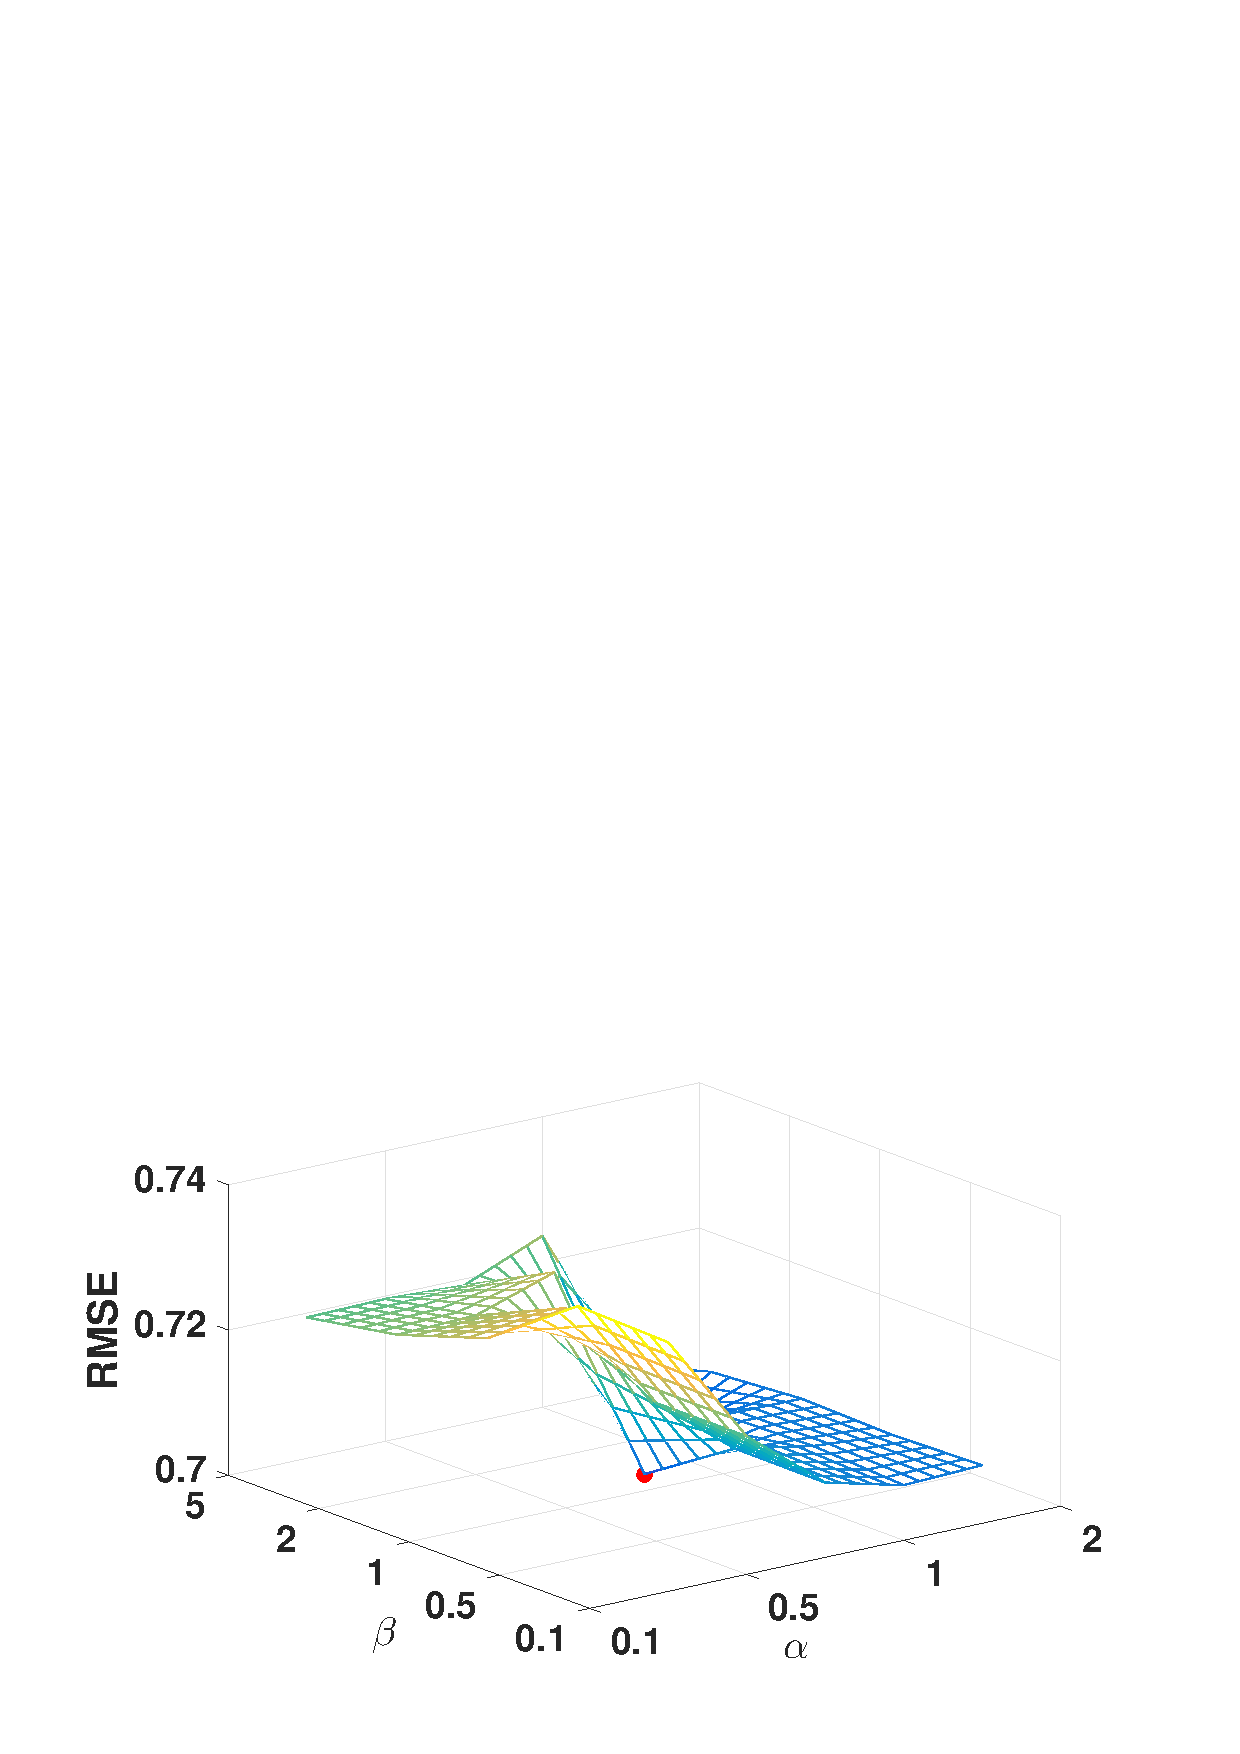
\includegraphics[width=8cm]{image/reg_rmse.pdf}
%\caption{\label{fig_reg}Varying parameters $\alpha$ and $\beta$ on Douban Movie dataset.}
%\end{figure}

%\begin{figure}[htbp]
%%\centering
%\subfigure[RMSE]{
%\begin{minipage}[t]{0.5\textwidth}
%\centering
%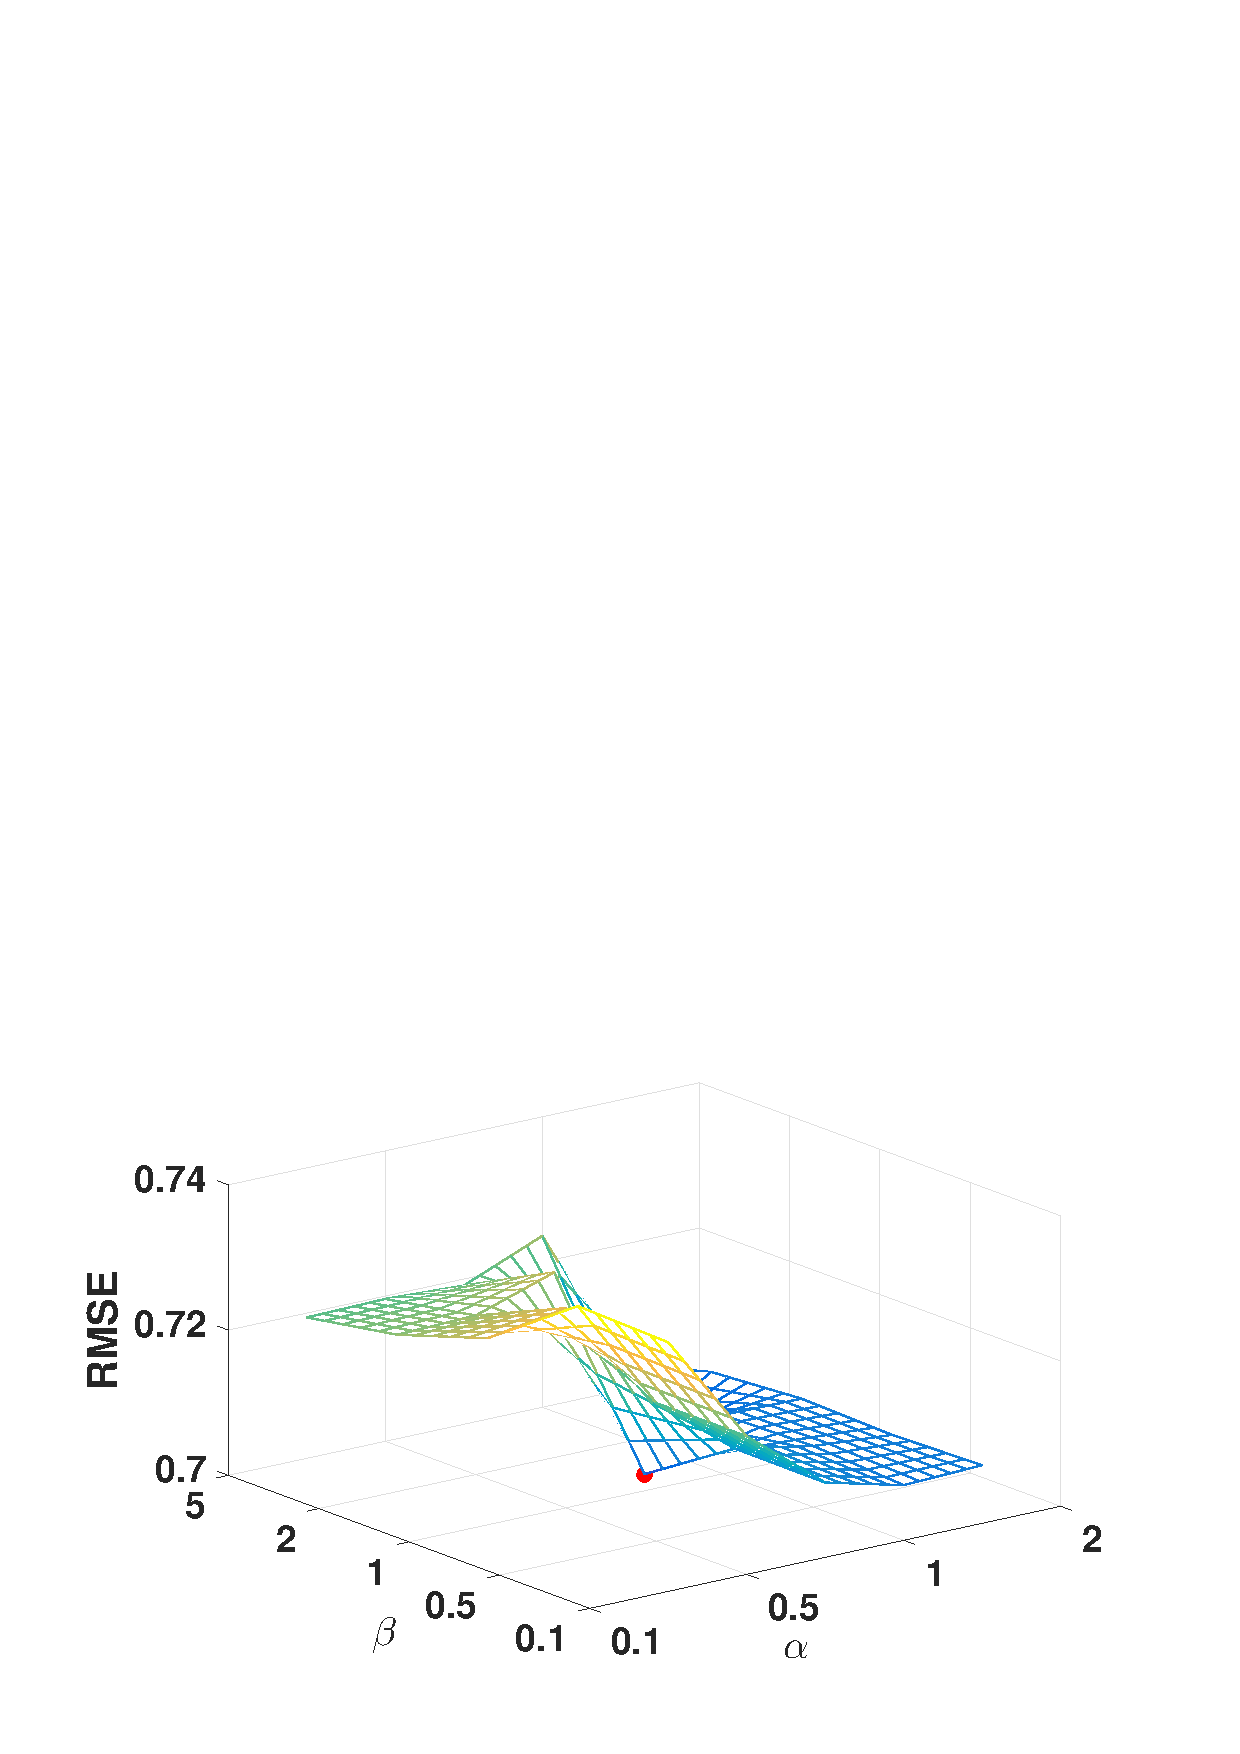
\includegraphics[width=8cm]{image/reg_rmse.pdf}
%\end{minipage}
%}
%\subfigure[MAE]{
%\begin{minipage}[t]{0.5\textwidth}
%\centering
%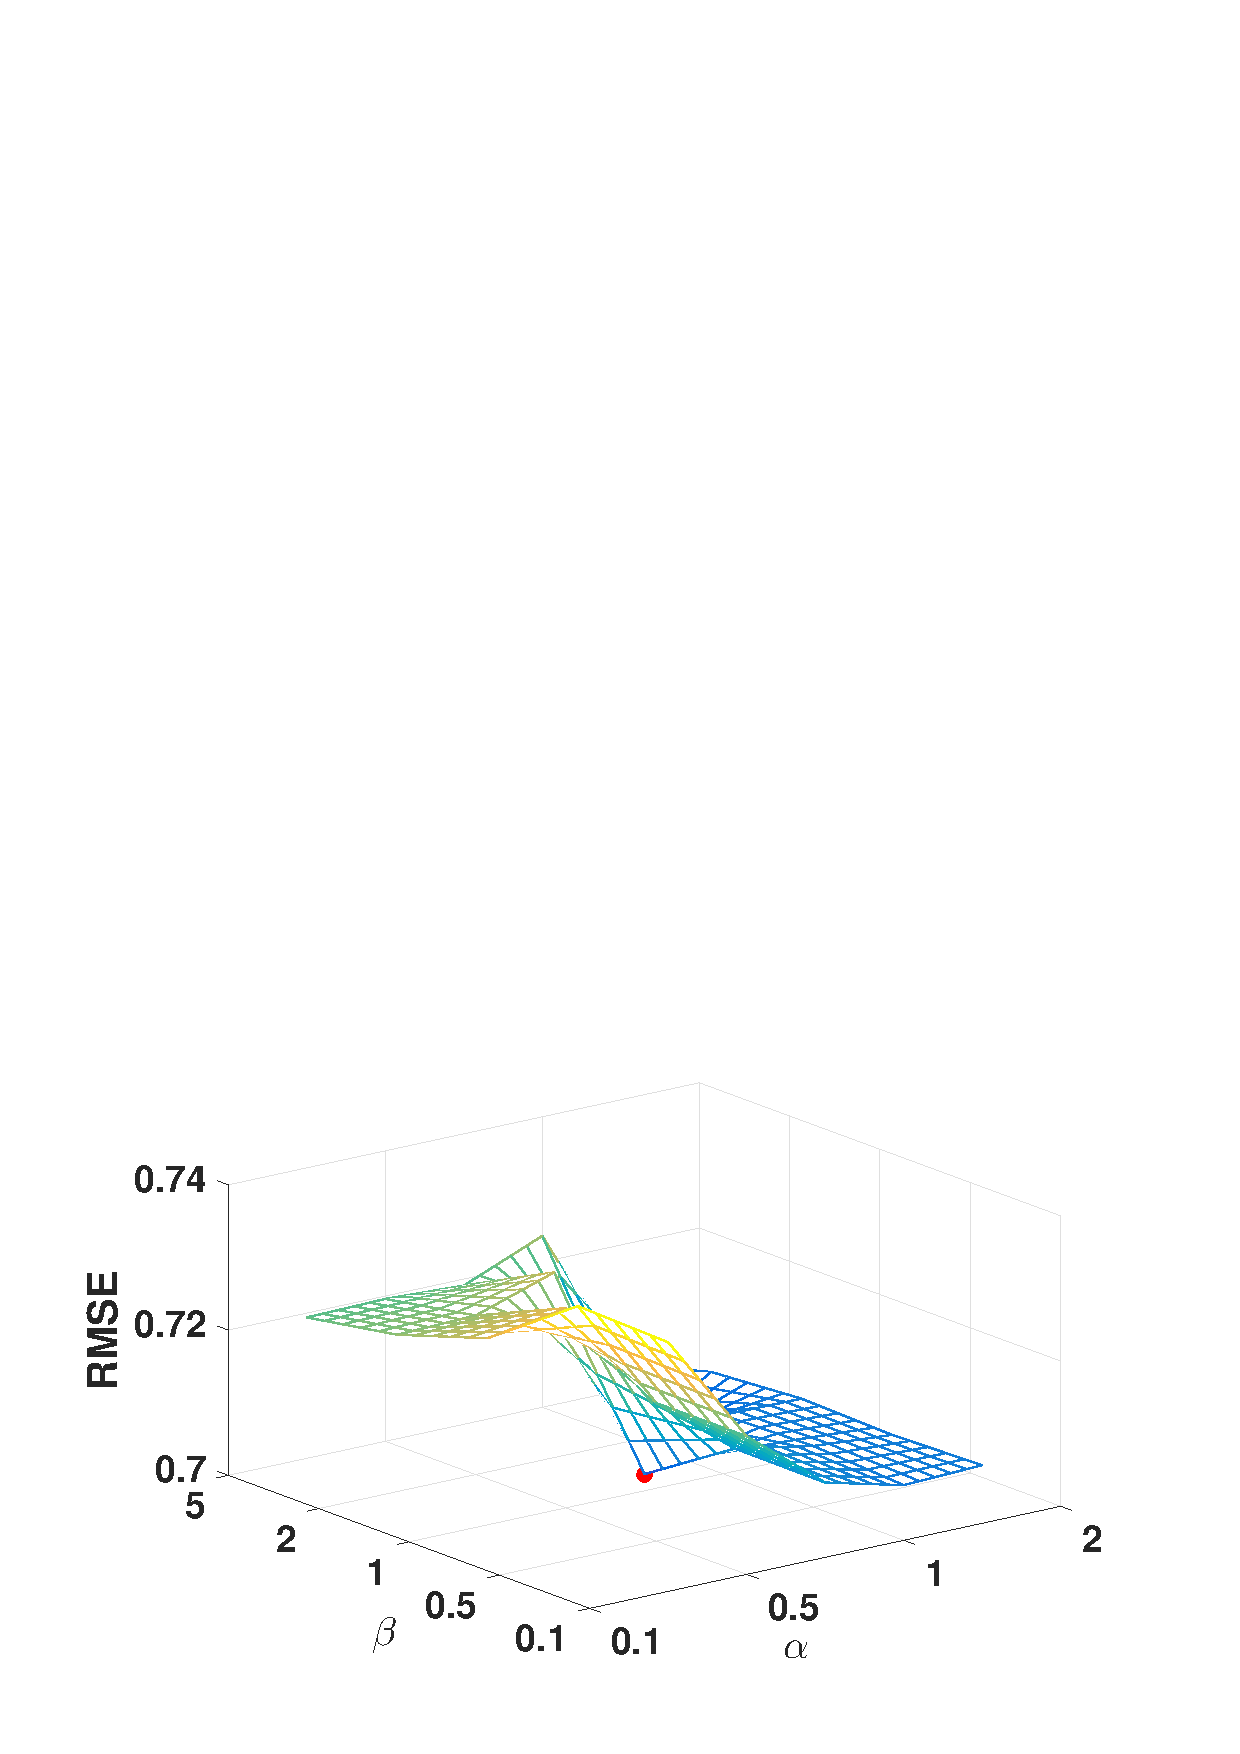
\includegraphics[width=8cm]{image/reg_rmse.pdf}
%\end{minipage}
%}
%\caption{\label{fig_reg}Varying parameters $\alpha$ and $\beta$ on Douban Movie dataset.}
%\end{figure}

\begin{figure*}[t]%[htbp]
\centering
\subfigure[Douban Movie]{
\begin{minipage}[t]{0.3\textwidth}
\centering
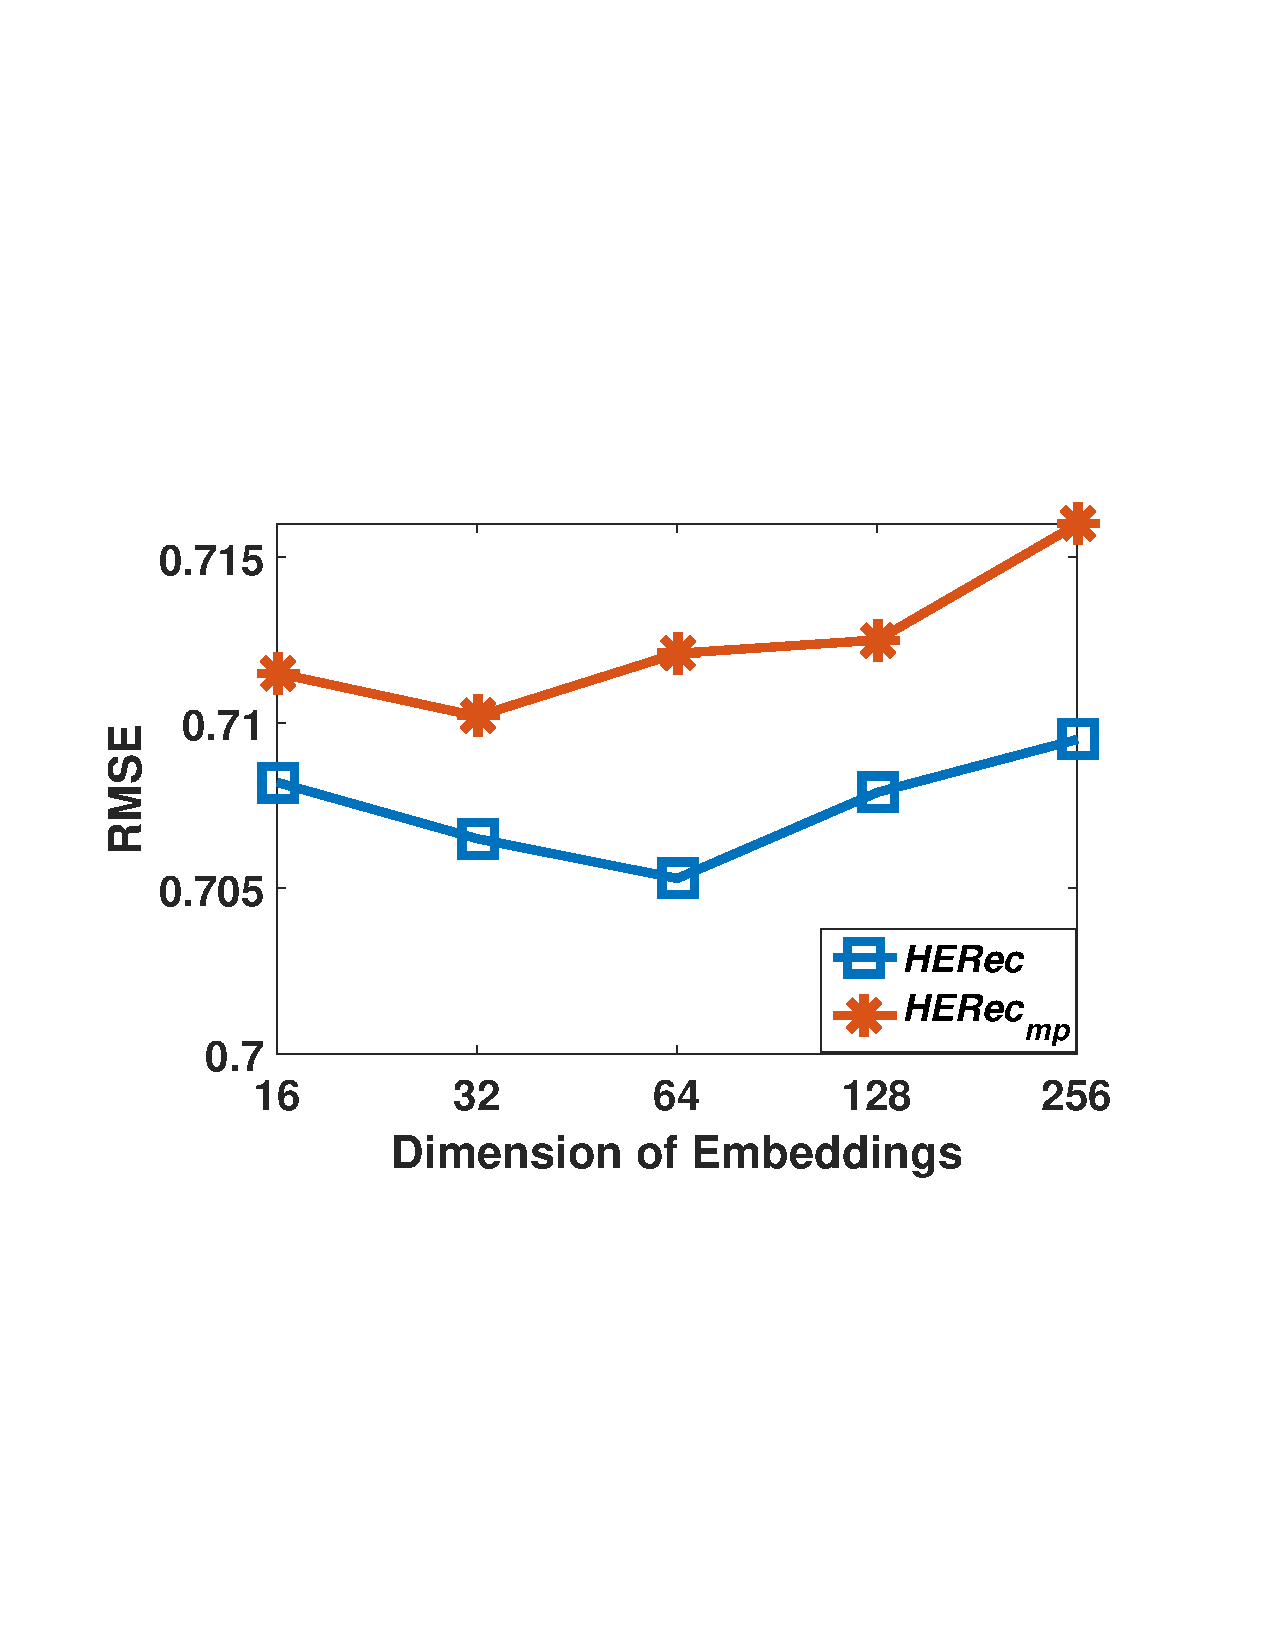
\includegraphics[width=1\textwidth]{image/dim_dm.pdf}
\end{minipage}
}
\subfigure[Douban Book]{
\begin{minipage}[t]{0.3\textwidth}
\centering
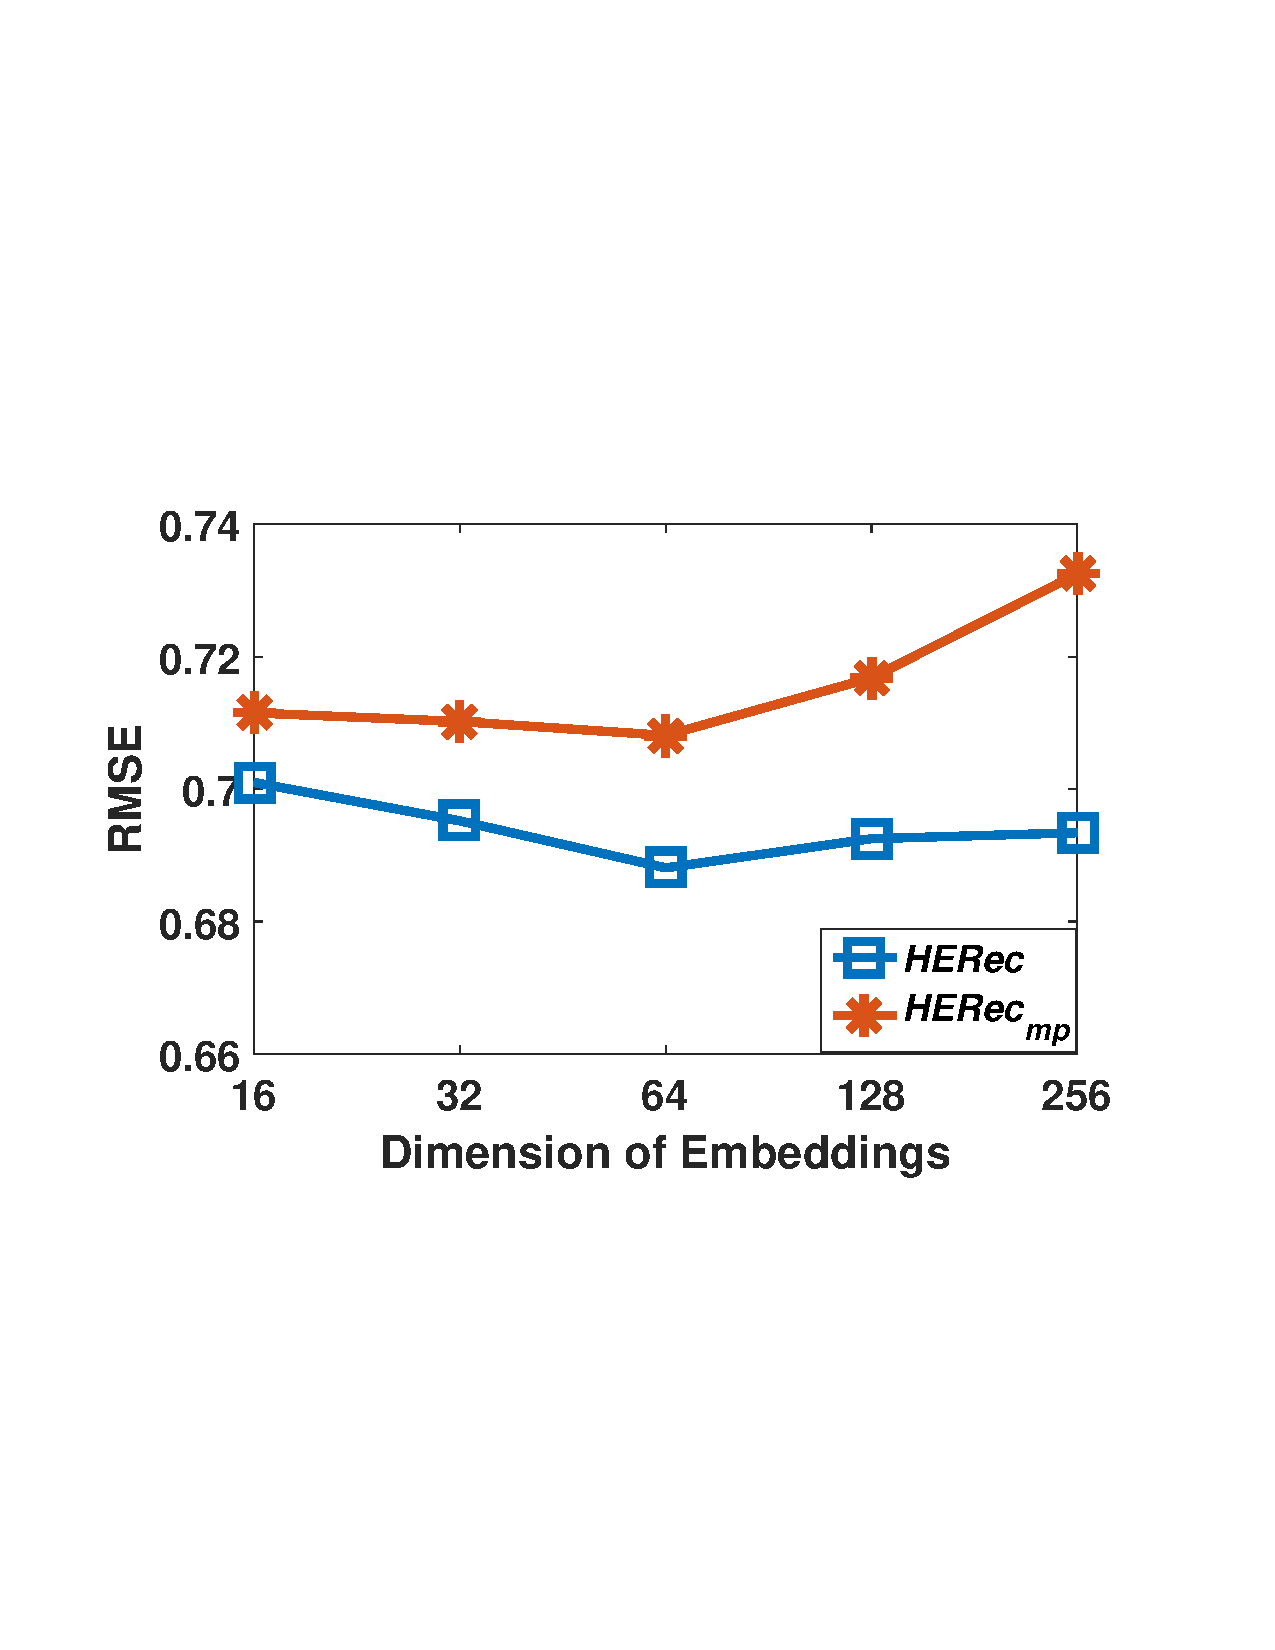
\includegraphics[width=1\textwidth]{image/dim_db.pdf}
\end{minipage}
}
\subfigure[Yelp]{
\begin{minipage}[t]{0.3\textwidth}
\centering
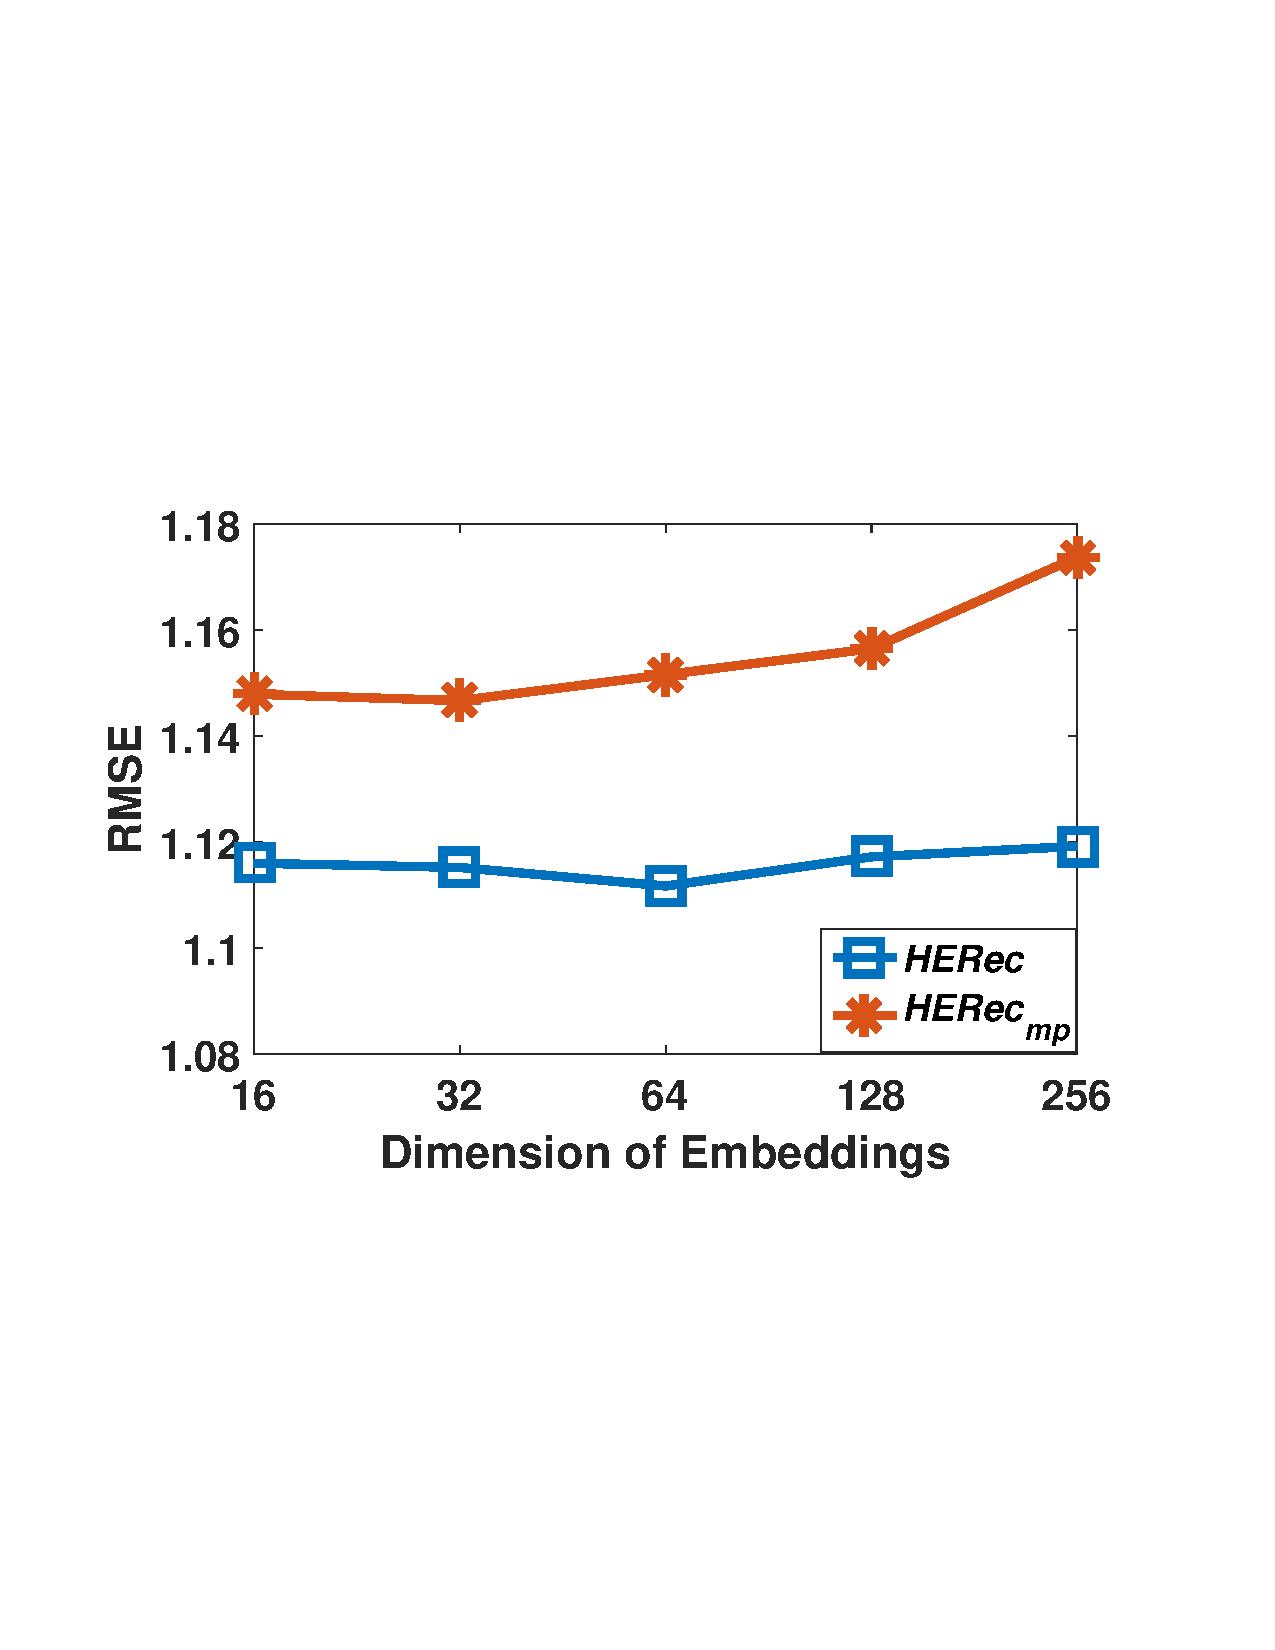
\includegraphics[width=1\textwidth]{image/dim_yelp.pdf}
\end{minipage}
}
\caption{\label{fig_dim}Performance change with respect to the dimension of embeddings on three datasets.}
\end{figure*}


\begin{figure*}[t]%[htbp]
\centering
\subfigure[Douban Movie]{
\begin{minipage}[t]{0.3\textwidth}
\centering
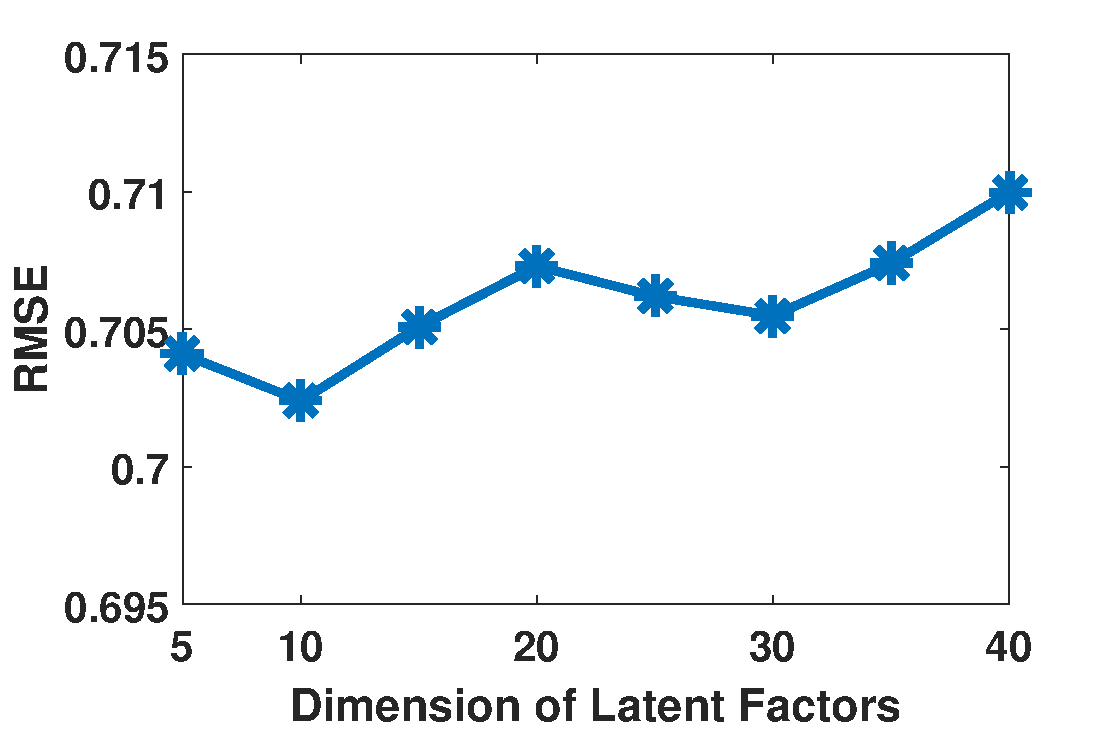
\includegraphics[width=1\textwidth]{image/factor_dm.pdf}
\end{minipage}
}
\subfigure[Douban Book]{
\begin{minipage}[t]{0.3\textwidth}
\centering
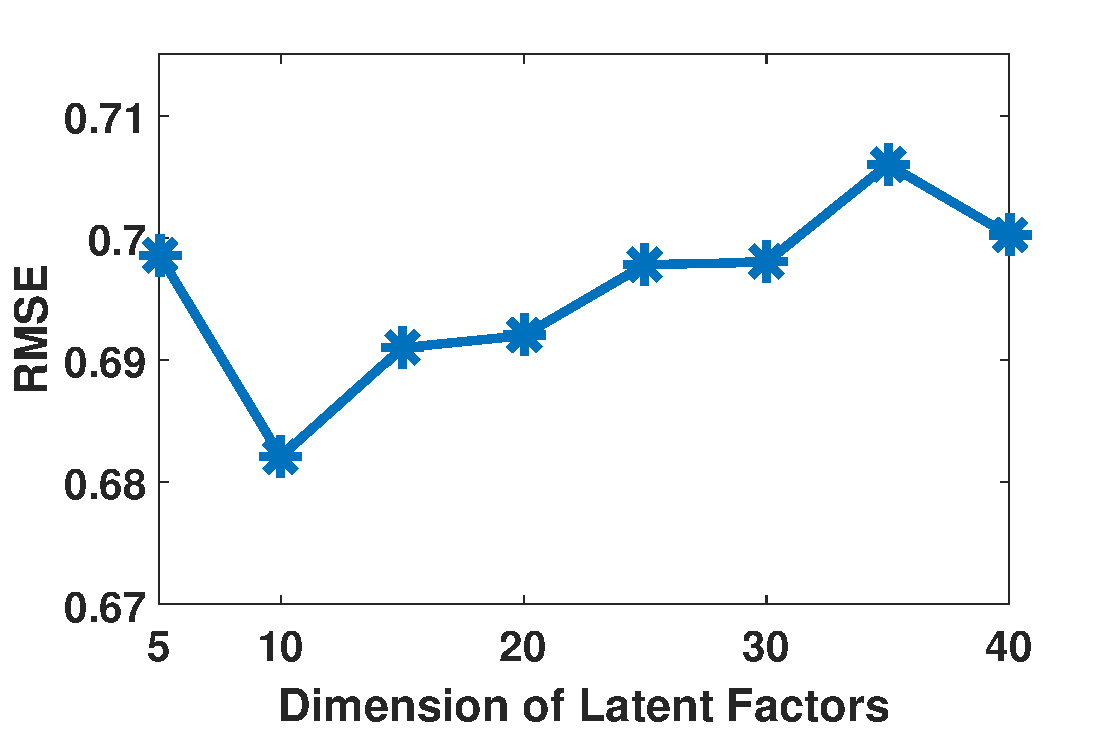
\includegraphics[width=1\textwidth]{image/factor_db.pdf}
\end{minipage}
}
\subfigure[Yelp]{
\begin{minipage}[t]{0.3\textwidth}
\centering
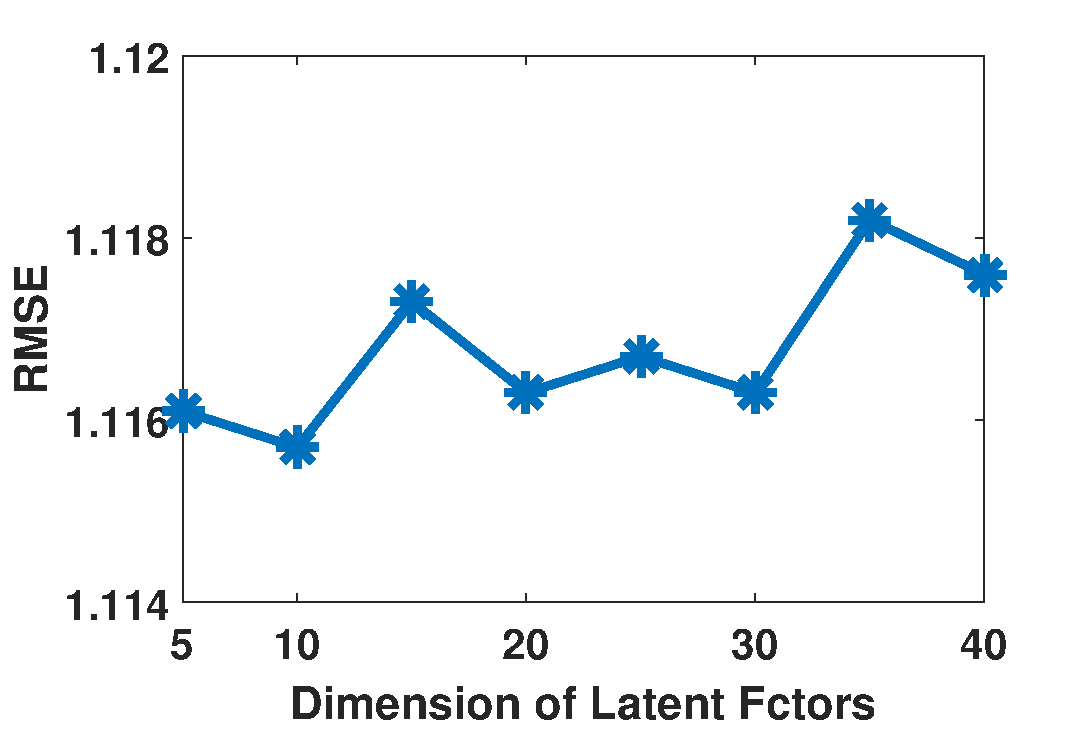
\includegraphics[width=1\textwidth]{image/factor_yelp.pdf}
\end{minipage}
}
\caption{\label{fig_factor}Performance change with respect to the dimension of latent factors on three datasets.}
\end{figure*}

\begin{figure*}[t]%[htbp]
\centering
\subfigure[Douban Movie]{
\begin{minipage}[t]{0.3\textwidth}
\centering
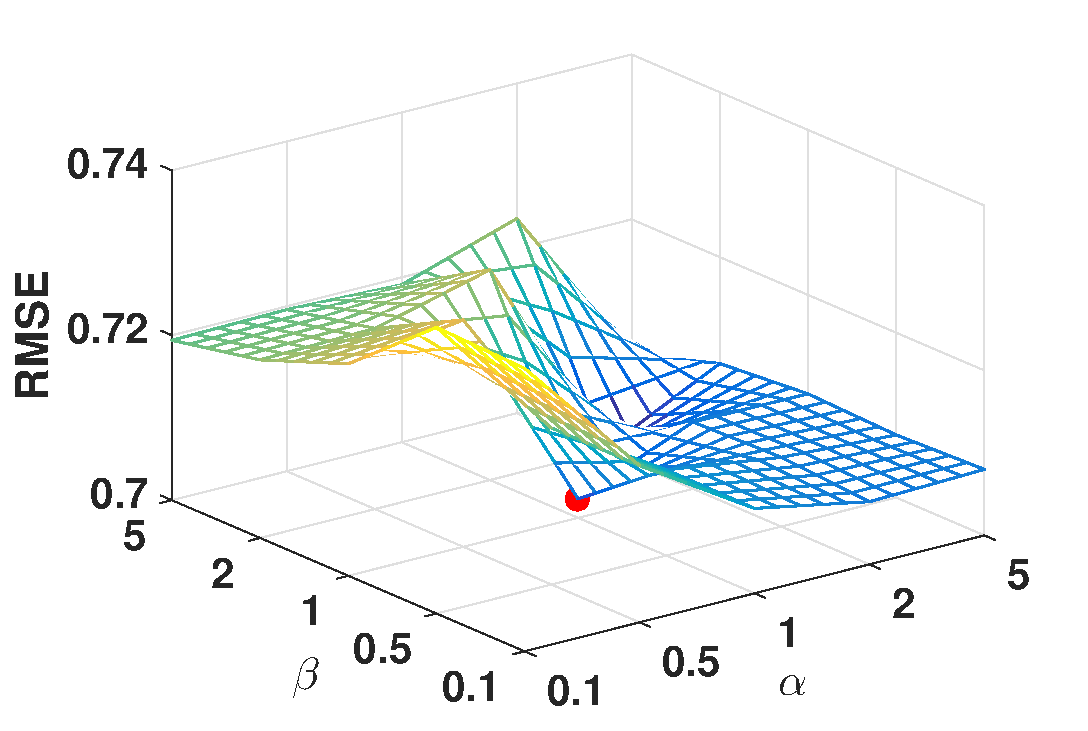
\includegraphics[width=1\textwidth]{image/reg_rmse_dm.pdf}
\end{minipage}
}
\subfigure[Douban Book]{
\begin{minipage}[t]{0.3\textwidth}
\centering
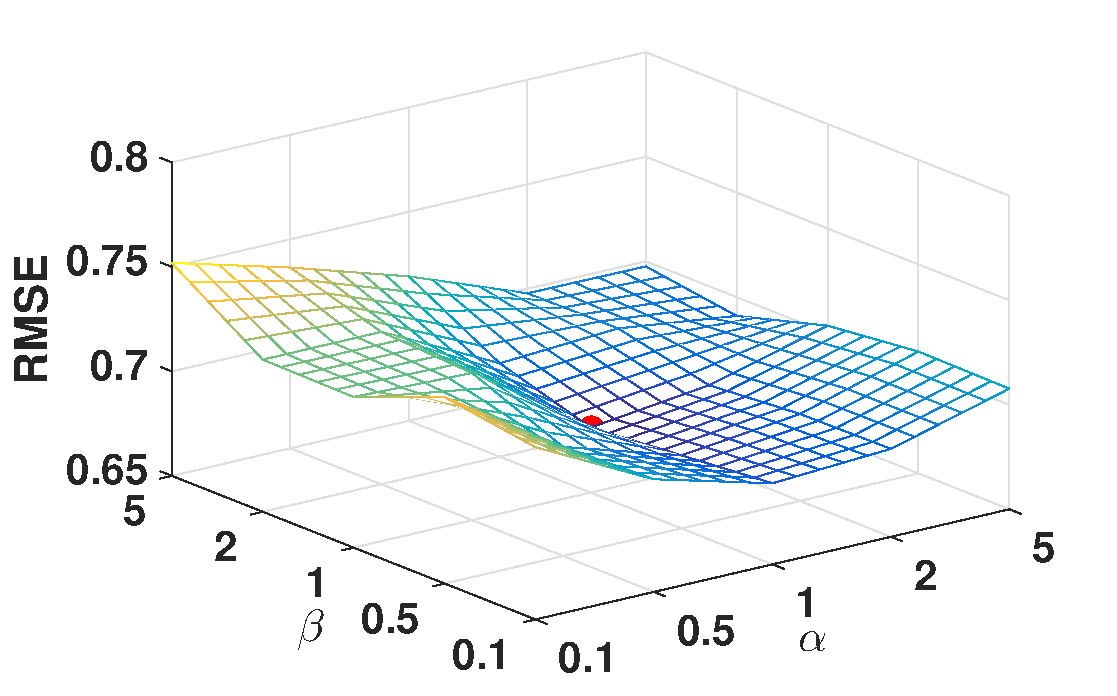
\includegraphics[width=1\textwidth]{image/reg_rmse_db.pdf}
\end{minipage}
}
\subfigure[Yelp]{
\begin{minipage}[t]{0.3\textwidth}
\centering
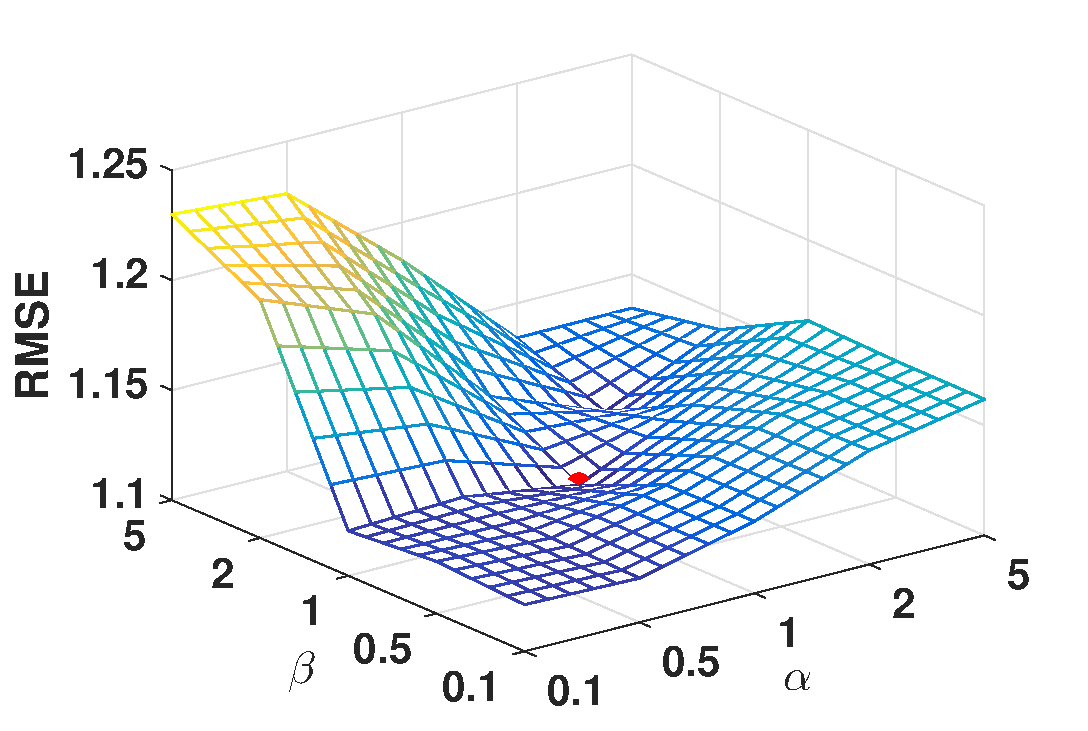
\includegraphics[width=1\textwidth]{image/reg_rmse_yelp.pdf}
\end{minipage}
}
\caption{\label{fig_reg}Varying parameters $\alpha$ and $\beta$ on the three datasets.}
\end{figure*}

%\begin{figure*}[t]%[htbp]
%\centering
%\subfigure[Douban Movie]{
%\begin{minipage}[t]{0.3\textwidth}
%\centering
%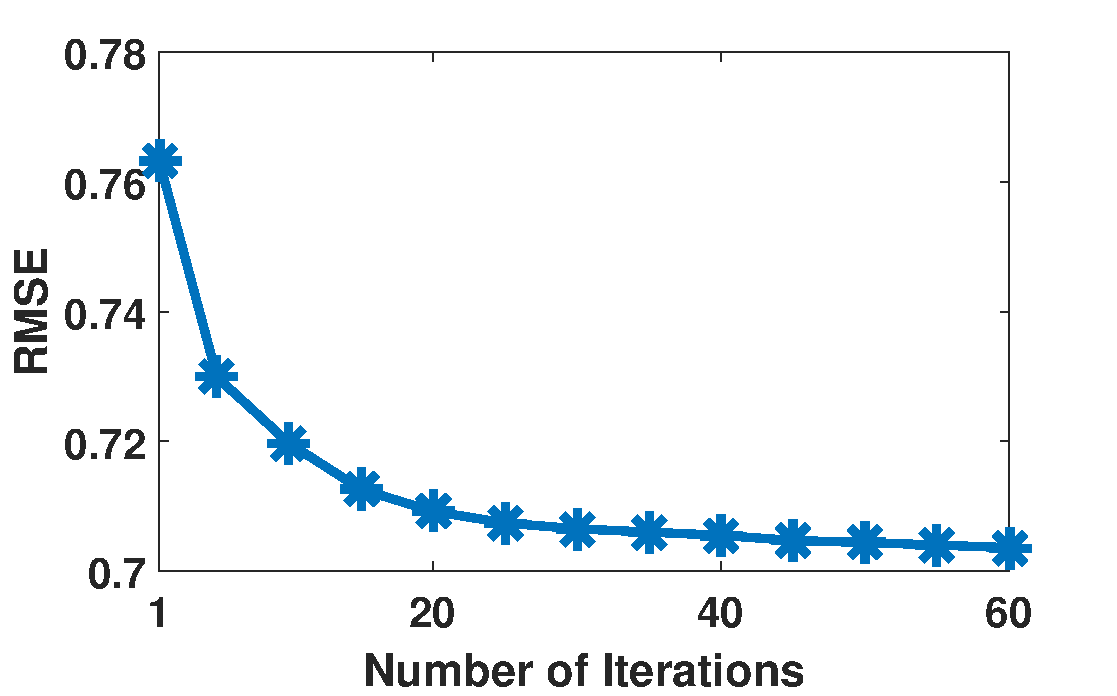
\includegraphics[width=1.06\textwidth]{image/iter_dm.pdf}
%\end{minipage}
%}
%\subfigure[Douban Book]{
%\begin{minipage}[t]{0.3\textwidth}
%\centering
%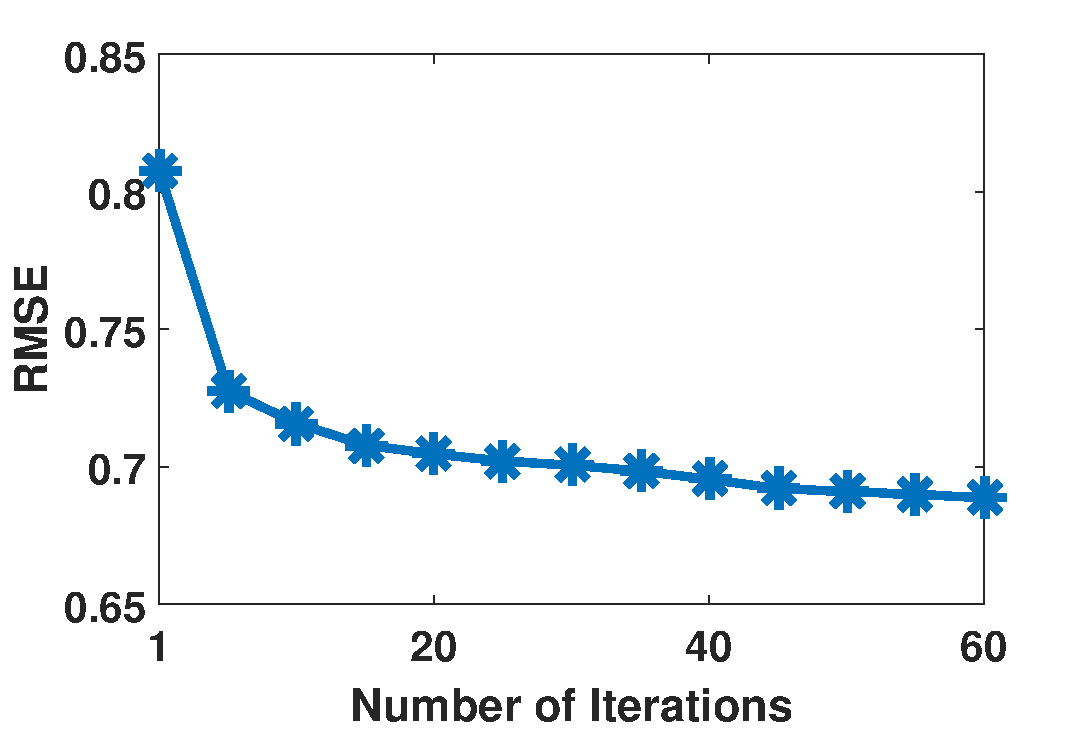
\includegraphics[width=1\textwidth]{image/iter_db.pdf}
%\end{minipage}
%}
%\subfigure[Yelp]{
%\begin{minipage}[t]{0.3\textwidth}
%centering
%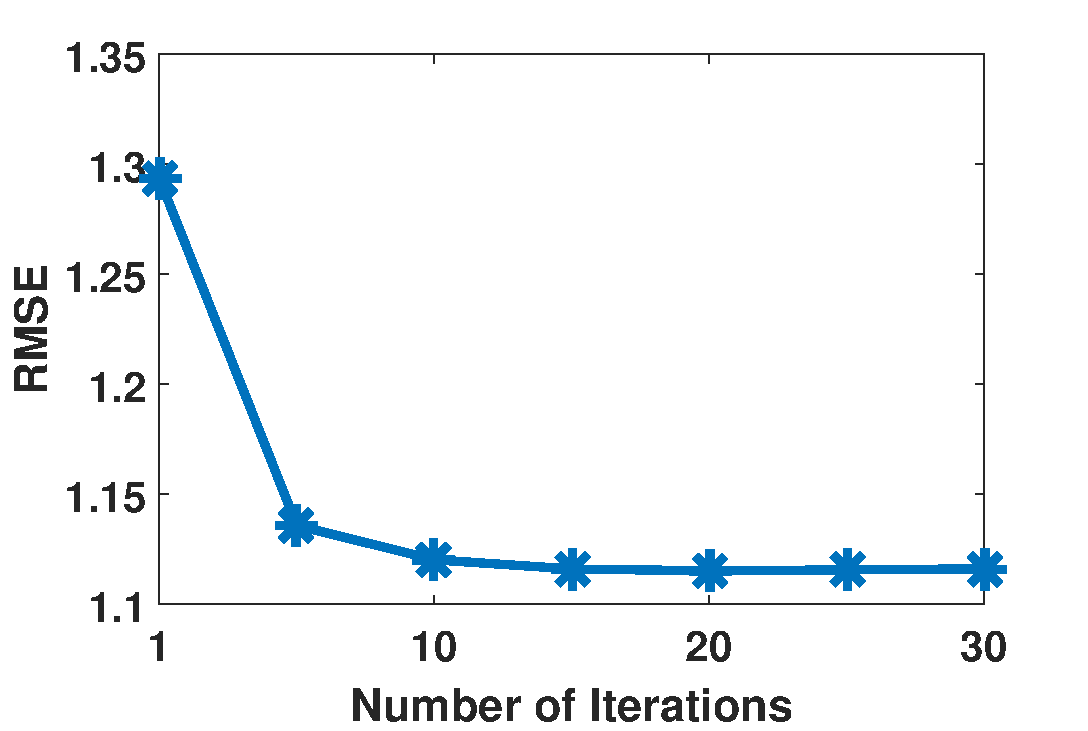
\includegraphics[width=1\textwidth]{image/iter_yelp.pdf}
%\end{minipage}
%}
%\caption{\label{fig_iter}Performance with respect to the number of iterations on three datasets.}
%\end{figure*}


\subsubsection{Parameter Tuning}
We firstly study the impact of the dimension of embeddings for the proposed model. We vary embedding dimensions in the set of $\{16, 32, 64, 128, 256\}$ and select HERec$_{mp}$ as the reference baseline. As shown in Fig.~\ref{fig_dim}, our method consistently outperforms HERec$_{mp}$ and achieves the optimal performance when the dimension of embeddings is around 64. Moreover, the performance of our method is more stable when varying the dimension of embeddings compared with HERec$_{mp}$.

For matrix factorization based methods, an important parameter to tune is the number of latent factors. The proposed model also involves such a parameter.
We vary it from 5 to 40 with a step of 5, and examine how the performance changes \emph{w.r.t} the number of latent factors.
We present the tuning results in Fig.~\ref{fig_factor}. As we can see, using 10 latent factors yields the best performance, indicating that
the number of latent factors should be set to a small number.

Next, we fix the number of latent factors as ten, and tune two other parameters $\alpha$ and $\beta$ (Eq.~\ref{eq-predictor}), which are used to integrate different terms as weights.
Now we examine how they influence the model performance. For both parameters, we vary them in the set of $\{0.1, 0.5, 1, 2\}$.
 As shown in Fig. \ref{fig_reg}, the optimal performance is obtained near $(1,1)$, \ie both $\alpha$ and $\beta$ are around 1. The results show that
 the HIN embeddings from both the user and item sides are important to improve the prediction performance.
 Overall, the change trend is smooth, indicating that the proposed model is not very sensitive to the two parameters.

 %Finally, we study the performance change \emph{w.r.t.} the number of iterations. As shown in Fig.~\ref{fig_iter},
 %we can see that the proposed model has a fast convergence rate, and about 40 to 60 iterations are required for dense datasets (\ie Douban Movie and Book), while about 20 iterations
 %are required for sparse datasets (\ie Yelp).
%
%\begin{figure}[htbp]
%%\centering
%\subfigure[RMSE]{
%\begin{minipage}[t]{0.5\textwidth}
%\centering
%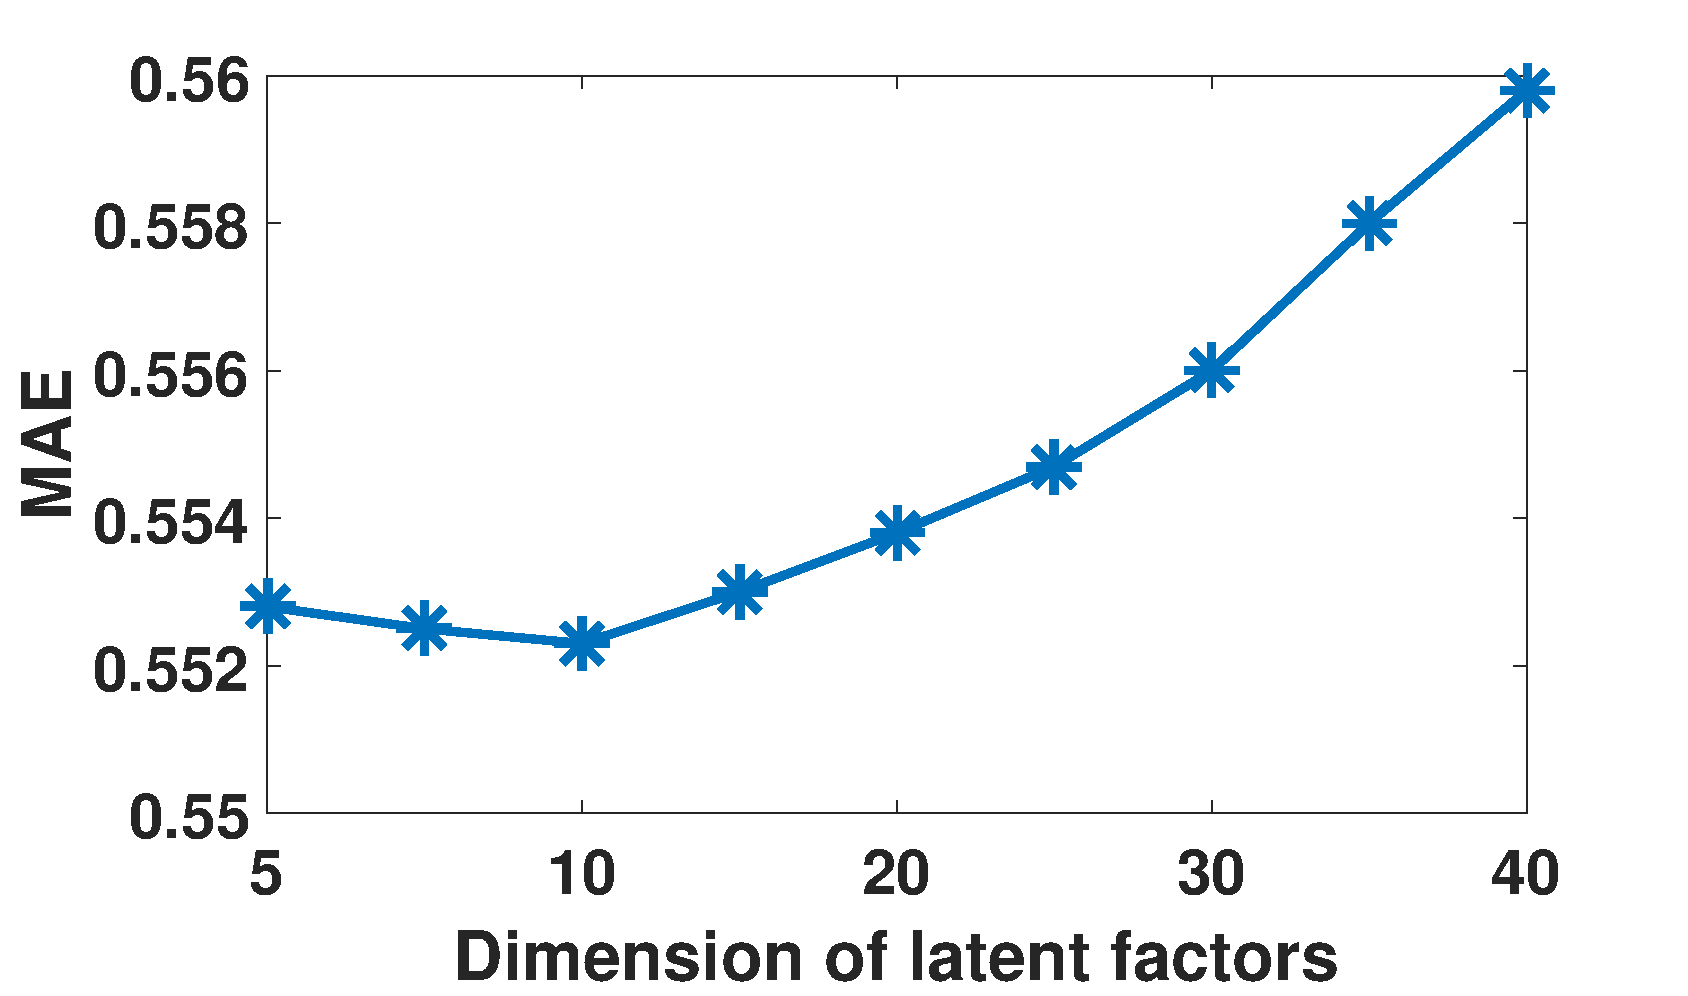
\includegraphics[width=8cm]{image/window_size_mae.pdf}
%\end{minipage}
%}
%\subfigure[MAE]{
%\begin{minipage}[t]{0.5\textwidth}
%\centering
%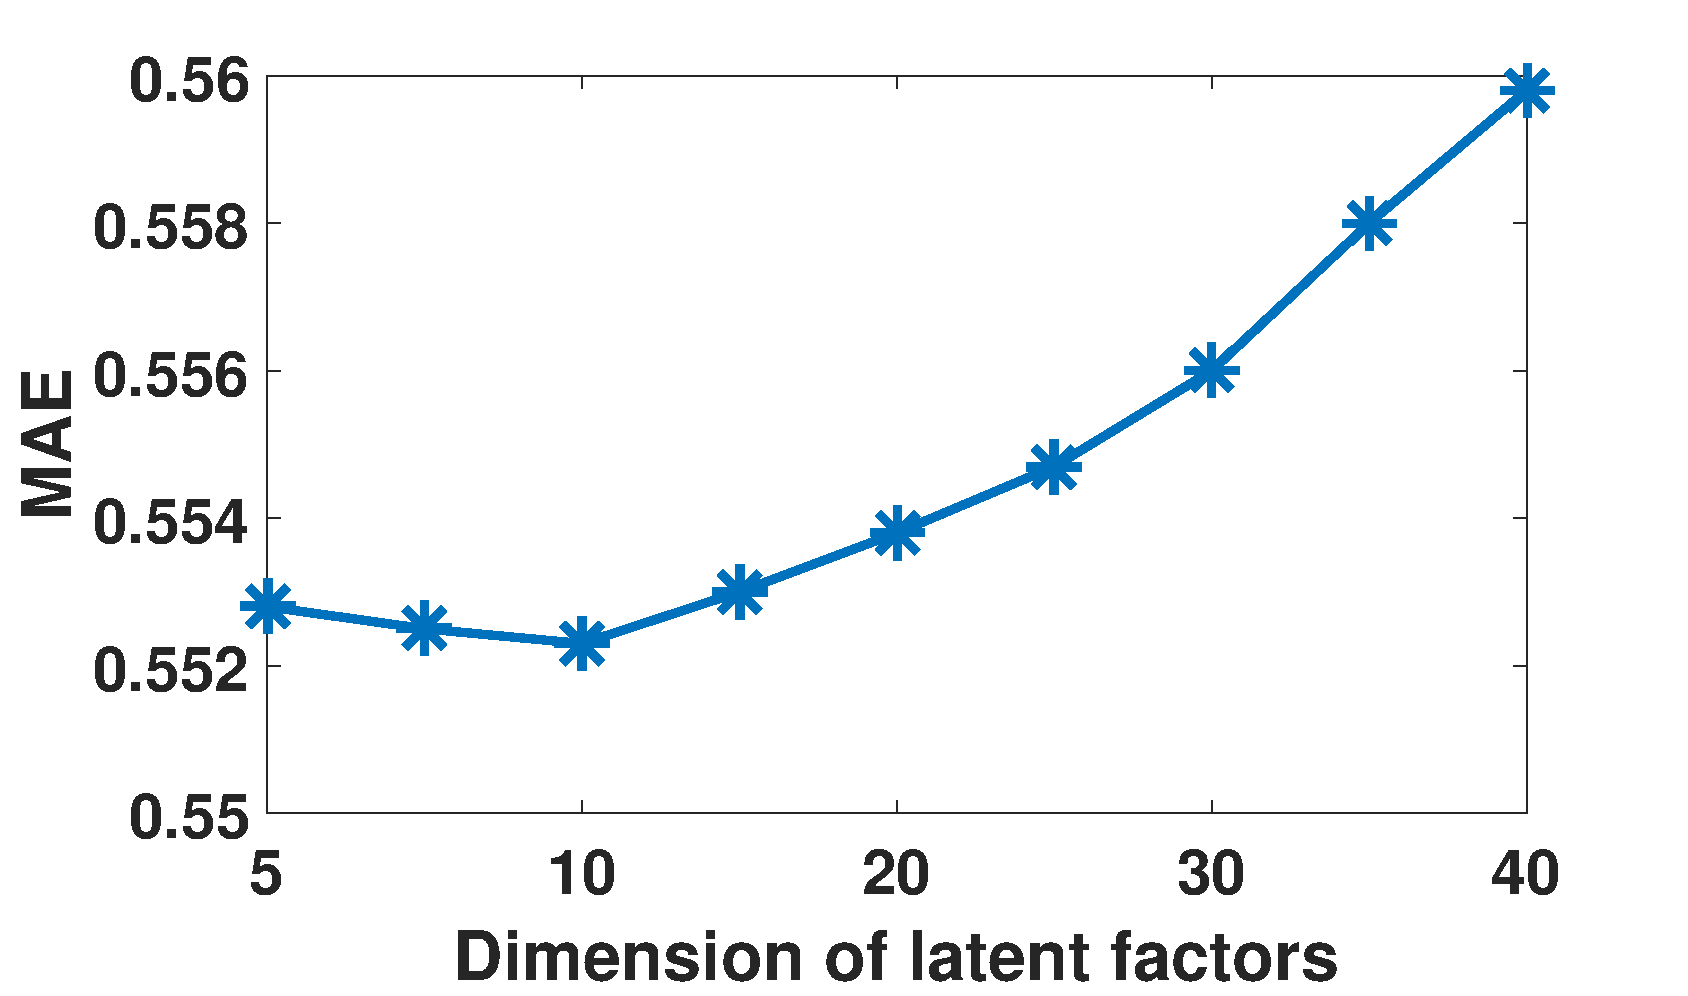
\includegraphics[width=8cm]{image/window_size_mae.pdf}
%\end{minipage}
%}
%\caption{\label{fig_reg}Dimension of latent factors.}
%\end{figure}

 %on Douban Movie dataset. As shows in Fig. \ref{fig_reg}, when the values of $\alpha$ and $\beta$ are both around 1, our model has the best performance. When the values of $\alpha$ and $\beta$ are quite large or small, the result is not good, especially in the case of small $\alpha$ and $\beta$. It shows that the latent features of users and items leant from HIN embedding both play an important role for better performances. However, too much weights on latent features of users and items also hurt the performances.
